\documentclass{report}

\usepackage[T1]{fontenc}
\usepackage[utf8]{inputenc}
\usepackage{times}

\usepackage[font=small,labelfont=bf,tableposition=top]{caption}
\usepackage{graphicx}
\usepackage{natbib} 

\usepackage{amsmath}
\usepackage{amsfonts}
\usepackage{amssymb}
\usepackage{color, soul}
\usepackage{hyperref}
\usepackage{algorithmicx}
\usepackage{algpseudocode}
\usepackage{subfigure}
\usepackage{stmaryrd}

\renewcommand{\vec}[1]{\boldsymbol{{#1}}} 
\newcommand{\duesoon}[1]{{\sethlcolor{green}\hl{#1}}}
\usepackage{mathrsfs}


\newtheorem{theorem}{Theorem}
\newtheorem{acknowledgement}[theorem]{Acknowledgement}
\newtheorem{algorithm}[theorem]{Algorithm}
\newtheorem{axiom}[theorem]{Axiom}
\newtheorem{case}[theorem]{Case}
\newtheorem{claim}[theorem]{Claim}
\newtheorem{conclusion}[theorem]{Conclusion}
\newtheorem{condition}[theorem]{Condition}
\newtheorem{conjecture}[theorem]{Conjecture}
\newtheorem{corollary}[theorem]{Corollary}
\newtheorem{criterion}[theorem]{Criterion}
\newtheorem{definition}[theorem]{Definition}
\newtheorem{example}[theorem]{Example}
\newtheorem{exercise}[theorem]{Exercise}
\newtheorem{lemma}[theorem]{Lemma}
\newtheorem{notation}[theorem]{Notation}
\newtheorem{problem}[theorem]{Problem}
\newtheorem{proposition}[theorem]{Proposition}
\newtheorem{remark}[theorem]{Remark}
\newtheorem{solution}[theorem]{Solution}
\newtheorem{summary}[theorem]{Summary}
\newenvironment{proof}[1][Proof]{\textbf{#1.} }{\ \rule{0.5em}{0.5em}}

\newtheorem{guess}{Definition}
\newcommand{\comment}[1] {}
\newcommand{\Norder} {N}
\newcommand{\order}{\mathcal{O}}
\newcommand{\Npoints} {N_p}
\newcommand{\Nfaces} {N_{f}}
\newcommand{\Nelements} {N_e}

\newcommand{\eps}{\varepsilon}
\newcommand{\Dweak}{\wt{D}}
\newcommand{\diff}[2] {\frac{\partial #1}{\partial #2}}
\newcommand{\dxx}[2] {\frac{\partial^2 #1}{\partial {#2}^2}}
\newcommand{\difft}[2] {\frac{d #1}{d #2}}
\newcommand{\dxxt}[2] {\frac{d^2 #1}{d {#2}^2}}
\newcommand{\lagrange}[1] {\frac{d #1}{dt}}
\newcommand{\lebesgue}{\parallel I \parallel}
\newcommand{\polysp}{\mathcal{P}_N}
\newcommand{\laplacian}{\nabla^2}
\newcommand{\divergence}{\nabla \cdot}
\newcommand{\inte}{\int_{\mbox{\footnotesize ${\Omega_e}$}}}
\newcommand{\intb}{\int_{\mbox{\footnotesize ${\Gamma_e}$}}}
\newcommand{\intce}{\int_{\mbox{\footnotesize ${\widehat{\Omega}_e}$}}}
\newcommand{\intcb}{\int_{\mbox{\footnotesize ${\widehat{\Gamma}_e}$}}}
\newcommand{\intg}{\int_{\mbox{\footnotesize ${\Omega}$}}}
\newcommand{\intgb}{\int_{\mbox{\footnotesize ${\Gamma}$}}}
\newcommand{\intv}{\int_{\mbox{\footnotesize ${\sigma}$}}}
\newcommand{\sumv}{\sum_{K=1}^{N_{\mathrm{lev}}}}
\newcommand{\sumk}{\sum_{L=1}^{K}}
\newcommand{\sumN}{\sum_{i=1}^{N+1}}
\newcommand{\half}{\frac{1}{2}}
\newcommand{\inti}{\int_{\mbox{\footnotesize\sf I}}}
\newcommand{\intbd}{\oint_{\mbox{\footnotesize ${\delta}$\sf D}}}
\newcommand{\intbi}{\oint_{\mbox{\footnotesize ${\delta}$\sf I}}}
\newcommand{\ldnorm}[1]{\left\| #1 \right\|_{\mbox{\footnotesize \sf D}} }
\newcommand{\lonorm}[1]{\left\| #1 \right\|_{\Omega}}
\newcommand{\spc}[1]{\mbox{\sf #1}}
\newcommand{\ope}[1]{{\cal #1}}
\newcommand{\mt}[1]{{\rm #1}}
\newcommand{\dis}{\displaystyle}
\newcommand{\ve}{\varepsilon}
\newcommand{\ov}{\overline}
\newcommand{\wt}{\widetilde}
\newcommand{\wh}{\widehat}
\newcommand{\Dhat}{\widehat{D}}
\newcommand{\be}{\begin{equation}}
\newcommand{\ee}{\end{equation}}
\newcommand{\bea}{\begin{eqnarray*}}
\newcommand{\eea}{\end{eqnarray*}}
\newcommand{\Jace}{J^{(e)}}
\newcommand{\Jacl}{J^{(l)}}
\def\bepsilon{\mbox{\boldmath $\epsilon $}}
\def\bpsi{\mbox{\boldmath $\psi $}}
\def\bphi{\mbox{\boldmath $\phi $}}
\def\bmu{\mbox{\boldmath $\mu $}}
\def\Et{ \tilde{E} }
\def\Ht{ \tilde{H} }
\def\sdot{ \dot{\sigma} }

\newcommand{\fstar}{f^{(*)}}

\DeclareMathOperator{\Span}{span}
\DeclareMathOperator{\Dim}{dim}

\newcommand{\polyquad}{\mathcal{Q}_{N}}
\newcommand{\polyP}{\mathcal{P}_{N}}
\newcommand{\polyPnpm}{\mathcal{P}_{(N+M)}}
\newcommand{\polyPd}{\mathcal{P}_{d}}
\newcommand{\polyPnm}{\mathcal{P}_{N,M}}
\newcommand{\polyPn}{\mathcal{P}_{N,0}}
\newcommand{\transpose}{^{\mathcal{T}}}

\newcommand{\vecQ}{\vec{Q}}
\newcommand{\vecQe}{\vec{Q}^{(e)}}
\newcommand{\vecFe}{\vec{\mathcal{F}}^{(e)}}
\newcommand{\statevec}{\vec{Y}}
\newcommand{\statevecN}{\vec{Y}_N^{(e)}}
\newcommand{\statestage}{\vec{\mathcal{Y}}}
\newcommand{\Ftensor}{\vec{F}(\qvector)}
\newcommand{\FtensorN}{\vec{F}\left( \qvectorN \right)}
\newcommand{\FtensorStar}{\vec{F}\left( \qvector_N^{(e,k)} \right)}
\newcommand{\Svector}{S(\qvector)}
\newcommand{\SvectorN}{S \left( \qvectorN \right)}
\newcommand{\qref}{\vec{q}_0}
\newcommand{\qvectorb}{\vec{q}_b}
\newcommand{\qtt}{\vec{q}_{tt}}
\newcommand{\qhat}{\widehat{\vec{q}}}
\newcommand{\qhatb}{\widehat{\vec{q}}_b}
\newcommand{\qelem}{q^{(e)}}
\newcommand{\rhoref}{\rho_0}
\newcommand{\piref}{\pi_0}
\newcommand{\Thetaref}{\Theta_0}
\newcommand{\Gref}{G_0}
\newcommand{\Tref}{T_0}
\newcommand{\thetaref}{\theta_0}
\newcommand{\Pref}{{P}_0}
\newcommand{\Eref}{{E}_0}
\newcommand{\Href}{{h}_0}
\newcommand{\rhohat}{\widehat{\rho}}
\newcommand{\pihat}{\widehat{\pi}}
\newcommand{\Phat}{\widehat{P}}
\newcommand{\uvechat}{\widehat{{\mbox{\boldmath$u$\unboldmath}}}}
\newcommand{\uhathat}{\widehat{\widehat{{\mbox{\boldmath$u$\unboldmath}}}}}
\newcommand{\Uhat}{\widehat{{\mbox{\boldmath$U$\unboldmath}}}}
\newcommand{\Uhathat}{\widehat{\widehat{{\mbox{\boldmath$U$\unboldmath}}}}}
\newcommand{\thetahat}{\widehat{\theta}}
\newcommand{\Thetahat}{\widehat{\Theta}}
\newcommand{\Ehat}{\widehat{E}}
\newcommand{\uhat}{\widehat{u}}
\newcommand{\vhat}{\widehat{v}}
\newcommand{\what}{\widehat{w}}
\newcommand{\pitt}{\pi_{tt}}
\newcommand{\rhott}{\rho_{tt}}
\newcommand{\Ett}{E_{tt}}
\newcommand{\Utt}{\vec{U}_{tt}}
\newcommand{\uvectt}{\vec{u}_{tt}}
\newcommand{\utt}{u_{tt}}
\newcommand{\vtt}{v_{tt}}
\newcommand{\wtt}{w_{tt}}
\newcommand{\Ptt}{P_{tt}}
\newcommand{\vecPtt}{\vec{P}_{tt}}
\newcommand{\Thetatt}{\Theta_{tt}}
\newcommand{\thetatt}{\theta_{tt}}
%Projector Matrices
\newcommand{\projmatrix}{\vec{\mathcal{P}}}
\newcommand{\qmatrix}{\vec{\mathcal{Q}}}
\newcommand{\pcmatrix}{\vec{\mathcal{P}}_C}
\newcommand{\Cmatrix}{\left(\vec{\mathcal{C}}^{(e,f)}\right)\transpose}
\newcommand{\Dmatrix}{\vec{D}^{(e)}}
\newcommand{\Dwmatrix}{\wt{\vec{D}}^{(e)}}
\newcommand{\Mmatrix}{M^{(e)}}
\newcommand{\Fmatrix}{\vec{F}^{(e,l)}}
\newcommand{\Gmatrix}{\mathcal{G}}
\newcommand{\Umatrix}{\mathcal{U}^{(e,f)}}
\newcommand{\amatrix}{\vec{\mathcal{A}}}
\newcommand{\rmatrix}{\vec{\mathcal{R}}}
%Vectors
\newcommand{\nvector}{\wh{\vec{n}}_{\Gamma}}
\newcommand{\nhat}{\wh{\vec{n}}}
\newcommand{\ivector}{\wh{\vec{i}}}
\newcommand{\jvector}{\wh{\vec{j}}}
\newcommand{\kvector}{\wh{\vec{k}}}
\newcommand{\rvector}{\wh{\vec{r}}}
\newcommand{\svector}{\wh{\vec{s}}}
\newcommand{\tvector}{\wh{\vec{t}}}
\newcommand{\vvector}{\wh{\vec{v}}}
\newcommand{\Qvector}{\vec{Q}}
%Vectors
\newcommand{\ur}{{u}^{(r)}}
\newcommand{\us}{{u}^{(s)}}
\newcommand{\ut}{{u}^{(t)}}
\newcommand{\urtt}{{u}_{tt}^{(r)}}
\newcommand{\ustt}{{u}_{tt}^{(s)}}
\newcommand{\uttt}{{u}_{tt}^{(t)}}
\newcommand{\urhat}{\widehat{u}^{(r)}}
\newcommand{\ushat}{\widehat{u}^{(s)}}
\newcommand{\uthat}{\widehat{u}^{(t)}}
%Other Operators
\newcommand{\grad}{\vec{\nabla}}
\newcommand{\Grad}{\vec{\nabla}}
\newcommand{\Dskew}{\mathcal{D}}

\def\bepsilon{\mbox{\boldmath $\epsilon $}}
\def\bpsi{\mbox{\boldmath $\psi $}}
\def\bphi{\mbox{\boldmath $\phi $}}
\def\bmu{\mbox{\boldmath $\mu $}}
\def\Et{ \tilde{E} }
\def\Ht{ \tilde{H} }
\def\sdot{ \dot{\sigma} }
%\renewcommand{\thetable}{\Roman{table}}
%\renewcommand{\thefigure}{\arabic{figure}}

%\DeclareMathOperator{\Span}{span}
%\DeclareMathOperator{\Dim}{dim}

%Editing Commands
\newcommand{\here}{ \textcolor{red}{YOU ARE HERE}}

%Time-Integration
\newcommand{\dt}{{\Delta t}}
\newcommand\ST{\rule[-0.75em]{0pt}{2em}}
\newcommand{\Sfunction}{\mathcal{S}}
\newcommand{\Lfunction}{\mathcal{L}}
\newcommand{\Nfunction}{\mathcal{N}}

%DG Operators
\newcommand{\average}[1]{ \left\{ #1 \right\} }
\newcommand{\jump}[1]{ \llbracket #1 \rrbracket }

%HDG Matrices
\newcommand{\CCmatrix}{\mathcal{C}^{(e,k)}}
\newcommand{\Jmatrix}{\mathcal{J}^{(e,k)}}
\newcommand{\DDmatrix}{\wt{D}^{(e)}}
\newcommand{\SSvector}{\mathcal{S}(q)}
\newcommand{\cghdg}{cg\underline{\hspace{0.15cm}}to\underline{\hspace{0.15cm}}hdg}
%\newcommand{\ul}{\underline{\hspace{0.15cm}}}
\newcommand{\RRmatrix}{\mathcal{R}}

%Clima specific variables
\newcommand{\etotal}{e^{\mathrm{tot}}}
\newcommand{\Etotal}{E^{\mathrm{tot}}}
\newcommand{\Fvector}{\vec{\mathcal{F}}}
\newcommand{\Pvector}{\vec{\mathcal{P}}}
\newcommand{\Fadv}{\vec{\mathcal{F}}^{\mathrm{adv}}}
\newcommand{\Fndf}{\vec{\mathcal{F}}^{\mathrm{ndf}}}
\newcommand{\Fdiff}{\vec{\mathcal{F}}^{\mathrm{diff}}}
\newcommand{\Tvector}{\vec{\mathcal{T}}}
\newcommand{\Source}{\vec{\mathcal{S}}}

\newcommand{\fxg}[1]{\textcolor{cyan}{FXG: #1}}


\usepackage[inline]{enumitem}

\title{CLIMA Numerics} 
\author{ }

\begin{document}

\maketitle
\tableofcontents

\chapter{Purpose, Goals, and Non-Goals}

\section{Overview}

This document describes the numerical methods implemented in the CLIMA models. It starts from a generic governing equation and lays out how it is discretized in space and in time. 

\section{Goals}

\begin{itemize}
    \item Provide a complete and self-contained documentation of the numerical methods available for CLIMA models, including space and time integration.
    \item Provide a summary of best practices in composing numerical methods for space and time discretization.
\end{itemize}

\section{Non-Goals}

\begin{itemize}
    \item Discuss details software architecture or data structures.
    \item Discuss implementation details such as variable names and computational aspects.
\end{itemize}
These are covered in the software design document \hl{[link]}.

%%%%%%%%%%%%%%%%%%%%%%%%%%%%%%%%%%% Governing Equations Chapter %%%%%%%%%%%%%%%%%%%%%%%%%%%%%%%%%%%%%%
\chapter{Governing Equations}\label{ch:gov_equations}

\section{Coordinate-Invariant Equations}

\subsection{Equations in Flux Form}

Abstractly, models such as the atmosphere, ocean, and land model consist of systems of balance equations of the form 
\begin{subequations}\label{e:balance_equations}
\begin{align}
     \frac{\partial}{\partial t} \rho + \nabla \cdot \left( \rho \vec{u} \right)
    & = \rho \mathcal{S}_\rho, \label{e:continuity}\\
   \frac{\partial}{\partial t} (\rho \vec{u})
    + \nabla \cdot \left( \rho (\vec{u} \otimes \vec{u} + \vec{\tau}) \right)
    & = \rho \vec{\mathcal{S}}_u,\\
     \frac{\partial}{\partial t} (\rho \theta) + \nabla \cdot \left(\rho (\vec{u}\theta + \vec{\mathcal{T}}) \right)
    & = \rho \mathcal{S}_\theta.
\end{align}
\end{subequations}
Here, $\otimes$ denotes the outer (Kronecker) product, and the following variables and functions of variables appear:
\begin{itemize}
    \item $\rho$: density;
    \item $\vec{u}$: 3D velocity vector;
    \item $\mathcal{S}_\rho$: mass source (per unit mass), e.g., owing to loss of water mass in precipitation;
    \item $\vec{\tau}$: specific momentum flux tensor owing to subgrid-scale (SGS) fluxes of momentum and (water) mass; $\vec{\tau}$ depends, for example, on the strain rate tensor; 
    \item $\Source_u$: specific momentum source vector, including, for example, pressure gradient, gravitational acceleration, and Coriolis accelerations, 
    \begin{equation}\label{e:momentum_source}
    \vec{\mathcal{S}}_u = -\frac{1}{\rho} \nabla p - \nabla\Phi - 2\vec{\Omega} \times \vec{u} + \vec{\mathcal{S}}'_u,
    \end{equation}
    where $\vec{\Omega}$ is the planetary angular velocity, $\Phi$ is geopotential, and $\vec{\mathcal{S}}'_u$ denotes all other momentum sources (e.g., the sink due to frictional drag);
    \item $\theta$: a generic scalar that stands symbolically for any of the several scalar variables in the model (e.g., for thermodynamic energy or water content);
    \item $\vec{\mathcal{T}}$: flux of scalar $\theta$ per unit mass, e.g., owing to SGS fluxes, which typically contains an SGS diffusion term
    \[
    \vec{\mathcal{T}} = - \vec{\mathcal{D}}_t \nabla \theta + \dots,
    \]
    with a symmetric but possibly anisotropic (and usually diagonal) turbulent diffusivity matrix $\vec{\mathcal{D}}_t$ (for example, $\vec{\mathcal{D}}_t$ may only have entries corresponding to vertical diffusion);
    \item $\mathcal{S}_\theta$: scalar source per unit mass, containing all terms responsible for non-conservation of $\theta$ (e.g., sources and sinks of water owing to precipitation formation in the atmosphere or owing to runoff in the soil model).
 \end{itemize}
 We split out the velocity vector $\vec{u}$ explicitly, rather than combining it with scalars into an abstract state vector, because it generally is the only true vector-valued state variable in the problem; other variables transform as scalars. 

Depending on the model, some terms and entire equations may not be present. For example, in the soil model, the density $\rho$ is constant and drops out. Additionally, the advective velocity $\vec{u}$ vanishes, so that the equations for the soil model reduce to balance equations for scalars $\theta$. The general formulation \eqref{e:balance_equations} is meant to encapsulate all of these different cases.

\subsection{Equations in Advective Form}

Using the continuity equation \eqref{e:continuity} to expand advective flux divergences in the balance equations for momentum and tracers yields the advective form of the governing equations:
\begin{subequations}\label{e:advective_equations}
\begin{align}
     \frac{\partial}{\partial t} \rho + \nabla \cdot \left( \rho \vec{u} \right)
    & = \rho \mathcal{S}_\rho, \\
     \frac{\partial}{\partial t} \vec{u} + \vec{u} \cdot \nabla \vec{u}
    & = \vec{\mathcal{S}}_u 
    - \frac{1}{\rho} \nabla \cdot \left(\rho \vec{\tau} \right) 
    - \vec{u} \mathcal{S}_\rho,\label{e:mom_advective}\\
     \frac{\partial}{\partial t} \theta + \vec{u} \cdot \nabla \theta 
    & = \mathcal{S}_\theta - \frac{1}{\rho} \nabla \cdot \left(\rho \vec{\mathcal{T}} \right) - \theta \mathcal{S}_\rho.
\end{align}
The continuity equation is left in flux form, as is common. The mass source per unit mass $\mathcal{S}_\rho$ appears on the right-hand side of all equations here because mass is not necessarily conserved (though deviations from mass conservation due to precipitation formation are small in Earth's atmosphere, of order $10^{-5}$, and are often neglected). 

An alternative form of the momentum equation in advective form results from using the vector identity
\begin{align*}
\vec{u} \cdot \nabla \vec{u} &= \nabla \left( \frac{\| \vec{u} \|^2}{2} \right) - \vec{u} \times (\nabla \times \vec{u})\\
&= \nabla K + \vec{\omega} \times \vec{u},
\end{align*}
where 
\[
\vec{\omega} = \nabla \times \vec{u}
\]
is the relative vorticity vector and
\[
K = \frac{1}{2} \| \vec{u} \|^2
\]
is the kinetic energy per unit mass. Using this transformation, the advective momentum equation \eqref{e:mom_advective} can alternatively be written as
\begin{equation}\label{e:mom_advect_vort}
    \frac{\partial}{\partial t} \vec{u} + (2\vec{\Omega} + \vec{\omega}) \times \vec{u}
    = -\frac{1}{\rho}\nabla p - \nabla (\Phi + K) + \vec{\mathcal{S}}'_u  
    - \frac{1}{\rho} \nabla \cdot \left(\rho \vec{\tau} \right) 
    - \vec{u} \mathcal{S}_\rho,
\end{equation}
\end{subequations}
where we have combined the term involving the relative vorticity $\vec{\omega}$ with the Coriolis acceleration $-2\vec{\Omega} \times \vec{u}$ in the source term $\vec{\mathcal{S}}_u$.

Hybrid equation sets are also commonly used. For example, it had been common for decades to use an advective form of the momentum equation, discretized with spectral methods, combined with flux forms of scalar equations, discretized with finite-volume methods. It can be advantageous to use the advective form of the momentum equation for discretization because it leads to a more accurate representation of wave modes and geostrophic balance than the flux form; however, using flux forms for the continuity and thermodynamic equations usually does not substantially affect dispersion characteristics of wave modes \citep{Thuburn05n}.

\section{Transformation to Generalized Coordinates}

\subsection{Coordinate System and Metrics}

To represent the governing equations in an arbitrary coordinate system, we need to express the various differential and vector operations appearing in the coordinate-invariant equations \eqref{e:balance_equations} or \eqref{e:advective_equations} in generalized coordinates. What follows is a  primer on standard results of vector and tensor analysis needed for coordinate transformations \citep[see, e.g.,][chapter~4]{Arfken13}.

We consider general (possibly nonorthogonal and curvilinear) coordinates $(\xi^1, \xi^2, \xi^3)$, with corresponding basis vectors 
\[
\vec{b}_1 = \frac{\partial \vec{r}}{\partial \xi^1}, \quad \vec{b}_2 = \frac{\partial \vec{r}}{\partial \xi^2}, \quad\vec{b}_3 = \frac{\partial \vec{r}}{\partial \xi^3},
\]
where $\vec{r}$ is a position vector. The basis vectors $\vec{b}_1$, $\vec{b}_2$, and $\vec{b}_3$ generally are neither unit vectors nor are they mutually orthogonal. For example, for spherical polar coordinates (which are orthogonal), we would choose longitude ($\xi^1 = \lambda$), latitude ($\xi^2 = \phi$), and radius ($\xi^3 = r$) as the coordinates. But for now, we consider completely general coordinates. Later we will specialize this to situations where $\xi^1$ and $\xi^2$ are horizontal coordinates and $\xi^3$ is a generalized vertical coordinate.

We will need the (symmetric) covariant metric tensor
\begin{equation}
    g_{ij} = \vec{b}_i \cdot \vec{b}_j = \frac{\partial x^k}{\partial\xi^i} \frac{\partial x^k}{\partial \xi^j},
\end{equation} 
where $\vec{r} = (x^1, x^2, x^3)$ denote coordinates of the position vector $\vec{r}$ in the reference frame in which the metric tensor is expressed. For example, they can be Cartesian coordinates of an embedding Euclidean reference space, or, on the sphere, they can be spherical polar coordinates. Here and throughout, we use the Einstein convention of summation over repeated indices. We also  adopt the usual convention that subscripts indicate covariant tensor components and superscripts contravariant tensor components \citep[e.g.,][]{Arfken13}. 

We will also need the contravariant metric tensor $g^{ij}$, which is the matrix inverse of the covariant metric tensor $g_{ij}$, that is, 
\[
g^{ik} g_{kj} = g_{jk} g^{ki} = \delta^i_j,
\]
where $\delta^i_j$ is Kronecker's delta (a mixed rank-2 tensor, as indicated by the raised and lowered indices). The Jacobian appearing in volume elements of the coordinate system is
\begin{equation}
    J = |\det g_{ij}|^{1/2};
\end{equation}
this is the Jacobian determinant $|\partial (x^1, x^2, x^3)/\partial (\xi^1, \xi^2, \xi^3)|$ (of the transformation from $(x^1, x^2, x^3)$ coordinates to $(\xi^1, \xi^2, \xi^3)$.

\subsection{Representation of Vectors and Tensors}

Consider generic vectors $\vec{F}$ (which may stand for the velocity $\vec{u}$, the momentum flux $\rho \vec{u}$, or the scalar flux $\rho \vec{u} \theta$) and generic rank-2 tensors $\vec{T}$ (which may stand for the specific momentum flux tensors $\rho \vec{u} \otimes \vec{u}$ or $\vec{\tau}$). In $(\xi^1, \xi^2, \xi^3)$ coordinates, they can be expressed as 
\begin{equation}\label{e:contravariant_vectors}
\vec{F} = F^i \vec{b}_i \quad \text{and} \quad \vec{T} = T^{ij} (\vec{b}_i \otimes \vec{b}_j), 
\end{equation}
where $F^i$ and $T^{ij}$ are the contravariant vector and tensor components. If needed, covariant vector components can be obtained by contraction of the covariant metric tensor with the contravariant components $F^j$ , for example,
\begin{equation}\label{e:covariant_components}
 F_i  = g_{ij} F^j = \vec{F} \cdot \vec{b}_i.
\end{equation}
Conversely, contravariant components $F^i$ can be obtained from the covariant components $F_j$ by contraction with the contravariant metric tensor
\begin{equation}
 F^i  = g^{ij} F_j.
\end{equation}

\subsection{Differential Operators}

To represent the equations \eqref{e:balance_equations} or \eqref{e:advective_equations} in $(\xi^1, \xi^2, \xi^3)$ coordinates, we need to express various differential operators in these coordinates. 

\paragraph{Gradient of a Scalar} The gradient of a scalar $\theta$ is a covariant vector, with components,
\[
(\nabla \theta)_i = \frac{\partial \theta}{\partial \xi^i}.
\]
Where we need the contravariant components of the gradient vector, we obtain them by contraction with the contravariant metric tensor,
\[
(\nabla \theta)^i = g^{ij} \frac{\partial \theta}{\partial \xi^j}.
\]

\paragraph{Gradient of a Vector (Covariant Derivative)} The derivative of a vector $\vec{F}$ with respect to the contravariant coordinates $\xi^j$ is
\begin{equation}
\begin{split}
\frac{\partial \vec{F}}{\partial \xi^j} & = \frac{\partial}{\partial \xi^j} (F^i \vec{b}_i)\\
& = \left( \frac{\partial F^i}{\partial \xi^j} +  \Gamma^i_{jk} F^k \right) \vec{b}_i.
\end{split}
\end{equation}
Here, the quantity in parentheses on the right-hand side is the covariant derivative, abbreviated $\nabla_j$,
\begin{equation}
    \nabla_j F^i = \frac{\partial F^i}{\partial \xi^j} +  \Gamma^i_{jk} F^k,
\end{equation}
where
\[
\Gamma^i_{jk} = \frac{g^{il}}{2} \left( \frac{\partial g_{jl}}{\partial \xi^k} + \frac{\partial g_{kl}}{\partial \xi^j} - \frac{\partial g_{jk}}{\partial \xi^l} \right)
\]
is the Christoffel symbol of the second kind, representing distortions of the coordinate system in space. The Christoffel symbols are defined by
\[
\frac{\partial\vec{b}_k}{\partial \xi^{j}} = \Gamma^{i}_{jk} \vec{b}_i
\]
and satisfy symmetry with respect to the lower indices, $\Gamma^{i}_{jk} = \Gamma^{i}_{kj}$.

\paragraph{Directional Derivative of a Scalar} The  directional derivative $\vec{u} \cdot \nabla \theta$ of a scalar $\theta$ is the contraction of the contravariant components $u^j$ of the direction vector $\vec{u}$ with the covariant gradient components,
\[
\vec{u} \cdot \nabla \theta = u^j \frac{\partial\theta}{\partial \xi^j}.
\]

\paragraph{Directional Derivative of a Vector} The contravariant components of the directional derivative $\vec{u} \cdot \nabla \vec{u}$ are given by the contraction of the contravariant components $u^j$ with the covariant derivative $\nabla_j u^i$,
\begin{align*}
(\vec{u} \cdot \nabla \vec{u})^i & = u^j \nabla_j u^i \\
& = u^j \frac{\partial u^i}{\partial \xi^j} + \Gamma^i_{jk} u^j u^k.
\end{align*}

\paragraph{Divergence of Vector} The divergence of a vector $\vec{F}$ can be written as 
\begin{equation}\label{eq:div-of-vec}
    \nabla \cdot \vec{F} = \frac{1}{J} \frac{\partial}{\partial \xi^j} \left(J {F}^j \right).
\end{equation}

\paragraph{Divergence of Tensor} The divergence of a contravariant rank-2 tensor $\vec{T}$ is  
\begin{align}\label{e:tensor_div}
(\nabla \cdot \vec{T})^i & = \nabla_j T^{ij} \\ 
&= \frac{1}{J} \frac{\partial}{\partial \xi^j} \left(J {T}^{ij} \right) + \Gamma^i_{jk} T^{jk}.
\end{align}

\paragraph{Curl} The contravariant components of the curl of a vector $\vec{F}$ are most easily written in terms of the covariant vector components $F_j$ as
\[
(\nabla \times \vec{F})^i = \frac{1}{J} \epsilon^{ijk} \frac{\partial F_k}{\partial \xi^j},
\]
where we used the completely antisymmetric Levi-Civita symbol 
\[
\epsilon_{ijk} = \epsilon^{ijk} = 
\begin{cases}
1 & \text{for $i$, $j$, $k$ even permutation of 1, 2, 3},\\
-1 & \text{for $i$, $j$, $k$ odd permutation of 1, 2, 3},\\
0 & \text{if any two indices are equal}.
\end{cases}
\]
Contraction with the covariant metric tensor can be used to obtain the covariant components of the curl, $(\nabla \times F)_i$, from the contravariant components $(\nabla \times \vec{F})^i$ according to  Eq.~\eqref{e:covariant_components}.

\subsection{Vector and Tensor Products}

\paragraph{Inner Product} The scalar (inner) product of two vectors $\vec{u}$ and $\vec{v}$ is 
\[
\vec{u} \cdot \vec{v} = u_i v^i = g_{ij} v^i u^j.
\]
This is used, for example, in the calculation of the specific kinetic energy $K = \| \vec{u} \|^2/2 = g_{ij} u^i u^j/2$.

\paragraph{Cross Product}
The covariant components of the vector cross product are
\[
(\vec{\Omega} \times \vec{u})_i = \epsilon_{ijk} \Omega^j u^k,
\]
and the corresponding contravariant components are obtained by contraction with the contravariant metric tensor,
\[
(\vec{\Omega} \times \vec{u})^i = g^{ij} \epsilon_{jkl} \Omega^k u^l.
\]

\paragraph{Outer Product} The contravariant outer (Kronecker) product is 
\[
(\vec{u} \otimes \vec{u})^{ij} = u^i u^j.
\]

\section{Equations in Generalized Coordinates}\label{e:EOM_general_coord}

\subsection{Equations in Flux Form}

Using the tensor identities above, we can represent the governing equations \eqref{e:balance_equations} in flux form in arbitrary coordinates $(\xi^1, \xi^2, \xi^3)$ as \citep[see, e.g.,][Appendix~A]{Kajishima17a}
\begin{subequations}\label{e:balance_equations_coord}
\begin{align}
 \frac{1}{J} \frac{\partial}{\partial t}  (\rho J) + \frac{1}{J} \frac{\partial}{\partial \xi^j} \left(\rho J u^j\right)
    & = \rho \mathcal{S}_\rho,\\
     \frac{1}{J}\frac{\partial}{\partial t} (\rho J u^i)
    + \nabla_j \left(\rho (u^i u^j +  \tau^{ij} ) \right)
    & = \rho \mathcal{S}^i_u,\\
    \frac{1}{J} \frac{\partial}{\partial t}  (\rho J \theta) + \frac{1}{J} \frac{\partial}{\partial \xi^j} \left(\rho J (u^j \theta + \mathcal{T}^j)\right)
    & = \rho \mathcal{S}_\theta.
\end{align}
Here, the covariant derivative $\nabla_j$ appears in the tensor divergence \eqref{e:tensor_div}, which written out is
\begin{equation}
\nabla_j \left(\rho (u^i u^j +  \tau^{ij} ) \right) =  \frac{1}{J} \frac{\partial}{\partial \xi^j} \left(\rho J (u^i u^j +  \tau^{ij}) \right) + \Gamma^i_{jk} \rho (u^j u^k +  \tau^{jk}).
\end{equation}
Unfortunately, (cumbersome) Christoffel symbols appear inside the tensor divergence in this equation set. 

We have expanded the four-dimensional space-time divergence on the left-hand sides as the coordinate-dependent form of the divergence. As a result, the Jacobian $J$ appears in the explicit time derivative because we want to allow vertical coordinates that are flow- and time-dependent (e.g., pressure based), in which case $J$ can be time-dependent. (It can be convenient to multiply the balance equations by $J$ and absorb the Jacobian into a new, coordinate-dependent density $\rho_\eta = \rho J$ \citep[e.g.,][]{Schneider03}.)  

Other differential operators such as gradients (e.g., pressure gradient) or vector operators such as cross products (e.g., the Coriolis acceleration) are inserted in the fluxes and source terms according to the transformation rules outlined above. For example, the terms associated with the pressure gradient, geopotential gradient, and Coriolis acceleration in the specific momentum source \eqref{e:momentum_source} become
\begin{equation}
\mathcal{S}_u^i  =  - g^{ij} \left( 
\frac{1}{\rho} \frac{\partial p}{\partial \xi^j} 
+ \frac{\partial \Phi}{\partial \xi^j}
+ \epsilon_{jkl} 2\Omega^k u^l \right) + \mathcal{S}_u^{'i}.
\end{equation}
\end{subequations}

It is evident that when using equations in flux form, contravariant velocity components $u^i$ are the natural ones to use. 

\subsection{Equations in Advective Form}

In advective form, using \eqref{e:mom_advect_vort} for the momentum equation, the equations for contravariant velocity components are
\begin{subequations}
\begin{align}\label{e:advective_equations_coord2}
 \frac{1}{J} \frac{\partial}{\partial t}  (\rho J) + \frac{1}{J} \frac{\partial}{\partial \xi^j} \left(\rho J u^j\right)
    & = \rho \mathcal{S}_\rho,\\
     \frac{\partial}{\partial t} u^i 
     + g^{ij} \epsilon_{jkl} (2\Omega^k + \omega^k) u^l 
    & = - g^{ij} \left(\frac{1}{\rho}\frac{\partial p}{\partial \xi^j} + \frac{\partial}{\partial \xi^j} (\Phi + K)  \right) \\
    & \qquad + \mathcal{S}^{'i}_u - \frac{1}{\rho} \nabla_j (\rho \tau^{ij}) - \mathcal{S}_\rho u^i,\\
    \frac{\partial}{\partial t} \theta + u^j \frac{\partial}{\partial \xi^j} \theta
    & = \mathcal{S}_\theta - \frac{1}{\rho J} \frac{\partial}{\partial \xi^j} \left(\rho J \mathcal{T}^j \right) - \theta \mathcal{S}_\rho,
\end{align}
where
\begin{equation}
    K = \frac{g_{kl} u^k u^l}{2}
\end{equation}
is the specific kinetic energy. 

Alternatively, the momentum equation can be written in terms of covariant velocity components as
\begin{multline}
    \frac{\partial}{\partial t} u_i + \epsilon_{ikl} (2\Omega^k + \omega^k) u^l 
    = \\
    -\frac{1}{\rho} \frac{\partial p}{\partial\xi^i}-  \frac{\partial}{\partial \xi^i} (\Phi + K) 
    + \mathcal{S}'_{u, i} - g_{ij} \frac{1}{\rho} \nabla_k (\rho \tau^{jk}) - \mathcal{S}_\rho u_i.\\
\end{multline}
Because in this form, the $i$-th covariant component of scalar gradients only involves derivatives with respect to $\xi^i$, it simplifies scalar gradients such as pressure and geopotential gradients. It can be exploited when two coordinates (e.g., $\xi^1$ and $\xi^2$) are purely horizontal; in that case, geopotential gradients only appear in one (vertical, $\xi^3$) equation, and only vertical derivatives appear in the equation for $u_3$.

As yet another alternative, the momentum equation can also be written with the full material derivative, 
\begin{multline}
\frac{\partial}{\partial t} u_i +  g_{ij} u^k\nabla_k u^j 
    + \epsilon_{ikl} 2\Omega^k u^l  =\\
     -\frac{1}{\rho} \frac{\partial p}{\partial\xi^i}-  \frac{\partial}{\partial \xi^i} \Phi 
    + \mathcal{S}'_{u, i}
     - g_{ij} \frac{1}{\rho} \nabla_k (\rho \tau^{jk}) - \mathcal{S}_\rho u_i.
\end{multline}
\end{subequations}
This form of the equation may be more convenient to use in non-rotating ($\vec{\Omega}=0$) situations. 

\section{Vertical Coordinates}

For a given radius $r$, the altitude 
\begin{equation}
    z = r - r_\mathrm{geo}(\lambda,\phi)
\end{equation}
is measured relative to the geoid, which has a radial distance $r_\mathrm{geo}(\lambda,\phi)$ from the barycenter of the planet. As is usually done, we approximate the planet as spherical, so that the geoid $r_\mathrm{geo}(\lambda,\phi) = a$ is taken to have a constant radius $a$, equal to the mean planetary radius. (However, it is not necessary to make this approximation, and at some point, it may be interesting to retain the fact that Earth is a rotational ellipsoid, with the geopotential gradient $\nabla \Phi$ being the normal to the geoid \citep{Baldauf20a}.)

It is common in atmosphere models to use terrain-following vertical coordinates $\xi^3=\eta$, defined such as that $\eta=0$ at the surface with elevation $z_s(\lambda, \phi)$, which depends on longitude $\lambda$ and latitude $\phi$ \citep{Kasahara74a}. Some common choices of terrain-following coordinates include:

\subsection{Gal-Chen and Sommerville Coordinate} \citet{Gal-Chen75a} offered one simple choice of a terrain-following coordinate, defined by 
\begin{equation}\label{e:Gal-Chen}
    r(\eta) = r_\mathrm{geo} + \eta z_t + z_s(\lambda, \phi)(1 - \eta),
\end{equation}
where $z_t$ is the vertical height of the domain, taken to be constant. This vertical coordinate is defined so that $\eta = 0$ at the surface ($z=z_s(\lambda, \phi)$) and $\eta = 1$ at the top ($z=z_t$) of the computational domain.

\subsection{Sch\"ar et al. Coordinate} \citet{Schar02a} introduced a terrain-following coordinate that gives stronger attenuation of the coordinate surface warping with height. This smooth-level vertical (SLEVE) coordinate is defined by
\begin{equation}\label{e:Schaer}
    r(\eta) = r_\mathrm{geo}(\lambda,\phi) +  \eta z_t + z_s(\lambda,\phi) \frac{\sinh\left((1-\eta)/s\right)}{\sinh(1/s)}.
\end{equation}
This vertical coordinate is likewise defined so that  $\eta = 0$ at the surface ($z=z_s(\lambda, \phi)$) and $\eta = 1$ at the top ($z=z_t$) of the computational domain (in a slight modification of the definitions of \citet{Schar02a}). The nondimensional scale $s$ gives an $e$-folding scale $s z_t$ over which the coordinate warping  decays with height. A typical choice for a computational domain with $z_t = 30~\mathrm{km}$ is $s=0.3$. For the coordinate to be well defined ($r$ must increase monotonically with $\eta$), it is crucial that the decay scale $s z_t$ is larger than the tallest topographic obstacle $\max(z_s)$. 

\citet{Schar02a} and \citet{Leuenberger10q} discuss how this vertical coordinate can be extended to a multiscale situation, in which the effects of smaller topographic scales on the coordinate surfaces decay more rapidly with height than those of larger scales.  

\subsection{Coordinate Stretching} \hl{[Describe how to stretch $\eta$ to increase resolution near the surface.]}

\subsection{Boundary Conditions} For the advective velocity $\vec{u}$, the physical no-slip boundary condition is generally unresolvable in GCMs and LES. The usual impenetrable (no normal flow) boundary conditions that instead are used at the top and bottom of the domain are 
\[
\vec{n} \cdot \vec{u} = 0 \qquad \text{at} \quad \eta = 0, 1,
\]
where $\vec{n}$ is the upward pointing unit normal vector at the boundary, with 
\[
\vec{n} = \frac{\nabla \eta}{\|\nabla \eta\|}. 
\]
Expanded in generalized coordinates, the covariant unit normal vector is
\[
n_i = \frac{1}{\|\nabla\eta\|} \frac{\partial\eta}{\partial \xi_i} \qquad \text{at} \quad \eta = 0, 1
\]
and with that, the no-normal flow condition in components becomes
\[
n_i u^i = 0.
\]

Similarly, we have boundary conditions on tracers $\theta$ themselves (which are unchanged in generalized coordinates from Cartesian coordinates) and on normal gradients of tracers, which appear in diffusive tracer fluxes, so that
\[
\vec{n} \cdot \nabla \theta = f \qquad \text{at} \quad \eta = 0, 1.
\]
Here, $f$ is some function given on the boundary. Expanded in generalized coordinates, this is 
\[
n_i g^{ij} \frac{\partial \theta}{\partial \xi^j} = f.
\]

\section{Example Coordinate Systems}\label{s:example_coordinates}

A few specific example coordinate systems to illustrate the relations above are the following.

\paragraph{Spherical Polar Coordinates} A common choice of coordinates are the polar spherical coordinates longitude ($\xi^1 = \lambda$), latitude ($\xi^2 = \phi$), and radius ($\xi^3 = r$). 
The transformation from Cartesian coordinates $(x, y, z)$ with origin at the center of the planet is
\begin{equation}
\label{e:spherical_polar_coordinates}
x = r\cos\phi\cos\lambda, \quad y = r\cos\phi\sin\lambda, \quad z = r\sin\phi.
\end{equation}
In this case, the Jacobian is
\[
J= r^2 \cos\phi,
\]
the coordinate system is orthogonal, and the metric tensors 
\begin{equation}\label{e:spherical_metric_tensors}
(g_{ij}) = \mathrm{diag}\left((r \cos\phi)^2, r^2, 1\right) 
\quad \text{and} \quad
(g^{ij}) = \mathrm{diag}\left((r \cos \phi)^{-2}, r^{-2},  1\right) 
\end{equation}
are diagonal.

We often use a local Cartesian system that is tangential to the sphere and in which the local Cartesian zonal velocity component is $u$ (eastward), the meridional velocity component is $v$ (northward), and the vertical velocity component is $w$ (upward). In terms of these velocities, the contravariant horizontal velocity components in spherical coordinates are the angular velocities 
\begin{equation}\label{e:angular_velocities}
u^1 = \frac{D\lambda}{Dt} = \frac{u}{r \cos\phi} \qquad \text{and} \qquad u^2 = \frac{D\phi}{Dt} = \frac{v}{r};
\end{equation}
the contravariant radial velocity is the vertical velocity 
\[
u^3 = \frac{Dr}{Dt} = w.
\]
Here, $D/Dt$ denotes the material derivative. The covariant velocities, obtained by contraction with the covariant metric tensor \eqref{e:spherical_metric_tensors}, are $(u_1, u_2, u_3) = (u r \cos\phi, r v, w)$.

\paragraph{Horizontal Cartesian Coordinates With Terrain-Following Vertical Coordinate} In LES settings with Cartesian geometry, we use horizontal Cartesian coordinates $x$ and $y$ and a terrain-following vertical coordinate $\eta$. 
The transformation from the Cartesian coordinates is
\[
x = x, \quad y = y, \quad z = z(x, y, \eta).
\]
In this case, the Jacobian determinant of transformation from Cartesian coordinates is 
\[
J = \frac{\partial z}{\partial\eta},
\]
and the covariant metric tensor is \citep{Guerra16a}
\begin{equation}\label{e:Cartesian_terrain_cov_metric}
    (g_{ij}) = \left(
    \begin{matrix}
    1 + \big(\frac{\partial z}{\partial x}\big)^{2} & 
    \frac{\partial z}{\partial x} \frac{\partial z}{\partial y} & 
    J \frac{\partial z}{\partial x}  \\
    & 
    1 + \big(\frac{\partial z}{\partial y}\big)^{2} 
    & J \frac{\partial z}{\partial y}  \\
     &
     & 
     J^2\\
    \end{matrix}
    \right),
\end{equation}
with the lower triangle completed by symmetry. The corresponding contravariant metric tensor is
\begin{equation}
    (g^{ij}) = \left(
    \begin{matrix}
    1 & 0 & - J^{-1} \left( \frac{\partial z}{\partial x} \right) \\
      & 1 & - J^{-1} \left( \frac{\partial z}{\partial y} \right) \\
      & & J^{-2} 
      \left[ 1 + \left( \frac{\partial z}{\partial x} \right)^2 + \left( \frac{\partial z}{\partial y} \right)^2 \right]
    \end{matrix}
    \right).
\end{equation}

% [Thank you!] \hl{no minus sign} $J^{-2} 
%      \left[ 1 + \left( \frac{\partial z}{\partial x} \right)^2 + \left( %\frac{\partial z}{\partial y} \right)^2 \right]$

The contravariant horizontal velocity components are the Cartesian velocity components 
\[
u^1 = \frac{Dx}{Dt} = u, \qquad u^2 = \frac{Dy}{Dt} = v
\]
in the $x$ and $y$ direction, respectively, and the velocity
\begin{align*}
u^3 & = \frac{D\eta}{Dt} 
 = \frac{\partial \eta}{\partial t} + u \frac{\partial \eta}{\partial x} + v \frac{\partial \eta}{\partial y} + w \frac{\partial \eta}{\partial z}\\
 & \equiv \dot \eta
\end{align*}
is the vertical velocity measured in the direction normal to surfaces of constant $\eta$ (i.e., normal to surface topography at the surface). The covariant velocity components follow by contraction with the covariant metric tensor \eqref{e:Cartesian_terrain_cov_metric}.

\paragraph{Spherical Polar Coordinates With Terrain-Following Vertical Coordinate} Another common choice of coordinates are the polar spherical coordinates longitude ($\xi^1 = \lambda$), latitude ($\xi^2 = \phi$), paired with a terrain-following vertical coordinate ($\xi^3 = \eta$). 
The transformation from Cartesian coordinates is
\[
x = r(\lambda, \phi, \eta)\cos\phi\cos\lambda, \quad y=r(\lambda, \phi, \eta)\cos\phi\sin\lambda, \quad z=r(\lambda, \phi, \eta)\sin\phi.
\]
In this case, the spherical coordinate system is no longer orthogonal. The Jacobian is \citep{Staniforth03a}
\[
J=  r^2 \cos\phi \, \frac{\partial r}{\partial \eta}.
\]
The covariant metric tensor $g_{ij}$ is 
\begin{equation}\label{e:spherical_terrain_cov_metric}
    (g_{ij}) = \left(
    \begin{matrix}
    r^2\cos\phi^2 + \big(\frac{\partial r}{\partial \lambda}\big)^2 &
    \frac{\partial r}{\partial \lambda}\frac{\partial r}{\partial \phi}& 
    \frac{\partial r}{\partial \lambda}\frac{\partial r}{\partial \eta} \\
   & 
   r^2 + \big(\frac{\partial r}{\partial \phi}\big)^2& 
   \frac{\partial r}{\partial \eta}\frac{\partial r}{\partial \phi} \\
       & & \big(\frac{\partial r}{\partial \eta}\big)^2
    \end{matrix}
    \right),
\end{equation}

The contravariant horizontal velocity components \eqref{e:angular_velocities} in a local Cartesian coordinate system are unchanged, but the contravariant vertical velocity is again the velocity
\[
u^3 = \frac{D\eta}{Dt} \equiv \dot\eta
\]
in the direction normal to surfaces of constant $\eta$. The covariant velocity components follow by contraction with the covariant metric tensor \eqref{e:spherical_terrain_cov_metric}.

For internal computations in the GCM, we use a similar coordinate system, but with coordinates on the faces of a cube parameterizing longitude $\lambda$ and latitude $\phi$ along spherical shells.

\section{Horizontal--Vertical Splitting of Equations}

Variations in the vertical in the climate system are usually much larger than variations in the horizontal. For example, in the soil, properties such as temperature and water content  in the vertical vary by $O(1)$ factors over scales of centimeters, but in the horizontal, they may vary by $O(1)$ factors only over tens of kilometers and more. Aspect ratios of mesh elements in a numerical model can reach $500:1$ in a global atmosphere model and $10^6:1$ in a land model. Hence, for numerical treatment of the equations, it is essential to split horizontal and vertical derivatives accurately. Otherwise, because quantities such as atmospheric pressure vary (exponentially) by $O(1)$ factors in the vertical on scales of kilometers, whereas horizontal variations even on planetary scales only are $O(10^{-2})$, calculations of horizontal pressure gradients become inaccurate, with large errors in large-scale dynamics. Additionally, splitting of the horizontal and vertical facilitates time stepping, for example, with implicit time discretization for vertical derivatives and explicit time discretization for horizontal derivatives. 

We can carry out this splitting using the representation of the equations in a generalized coordinate system. To be concrete, let's start from a specific set of governing equations, stated in coordinate-independent form. 

\subsection{Specification of Governing Equations}

As an example, we use the following governing equations in coordinate-invariant form,
\begin{subequations}\label{e:EOM_ex}
\begin{align}
     \frac{\partial}{\partial t} \rho + \nabla \cdot \left( \rho \vec{u} \right)
    & = \rho \mathcal{S}_\rho,  \\
    \frac{\partial}{\partial t} \vec{u} + (2\vec{\Omega} + \vec{\omega}) \times \vec{u}
    & = -\frac{1}{\rho} \nabla p - \nabla(\Phi + K) \nonumber \\
    & \qquad + \vec{\mathcal{S}}'_u - \frac{1}{\rho} \nabla \cdot \left(\rho \vec{\tau} \right) 
    - \vec{u} \mathcal{S}_\rho, \\
    \frac{\partial}{\partial t} (\rho \theta) + \nabla \cdot \left(\rho (\vec{u}\theta + \vec{\mathcal{T}}) \right)
    & = \rho \mathcal{S}_\theta.
\end{align}
\end{subequations}
That is, we use scalar equations in flux form and the momentum equation in advective form, with vorticity in the advection term.

For the user interface for specifying the governing equations, it will be advantageous to further split differential operators into vertical and horizontal components, e.g., $\nabla \cdot (\rho \vec{u}) = \nabla_h \cdot (\rho \vec{u}_h) + \nabla_z \cdot (\rho w \vec{k})$, where subscripts $h$ and $z$ denote horizontal and vertical components, and $\vec{k}$ is a vertical unit vector. The reason is that vertical flux terms will be treated separately in the timestepping from horizontal terms. \hl{[but we can also do this on the level of the coordinate-dependent equations, and it's better there---just how do you specify the splitting for sound and gravity waves at the API level then?]}

\subsection{Expansion in Generalized Coordinates}

To expand the equations in a set of coordinates, let $\xi^1$ and $\xi^2$ denote two horizontal coordinates. For example, they may be the Cartesian coordinates $\xi^1 = x$ and $\xi^2 =y$ for a model defined in Cartesian geometry; or they may be cubed-sphere coordinates parameterizing the polar coordinates longitude $\lambda$ and latitude $\phi$ for a model defined on a sphere. Let $\xi^3$ denote an arbitrary vertical coordinate, for example, the radial coordinate $r$ or a terrain-following coordinate $\eta$. 

To expand the governing equations in $(\xi^1, \xi^2, \xi^3)$ coordinates, we use the general relations in section~\ref{e:EOM_general_coord}. We want the coordinate-dependent equations to split as cleanly as possibly into vertical and horizontal momentum equations, to facilitate, for example, using implicit solves on vertical momentum equations without having to involve horizontal momentum equations. We achieve such a split using equations for the covariant velocities $u_1$ and $u_2$ in the horizontal and $u_3$ in the vertical. The governing equations in  $(\xi^1, \xi^2, \xi^3)$ coordinates become
\begin{subequations}
\begin{align}\label{e:equations_coord_hor_vert}
 \frac{1}{J} \frac{\partial}{\partial t}  (\rho J) + \frac{1}{J} \frac{\partial}{\partial \xi^j} \left(\rho J u^j\right)
    & = \rho \mathcal{S}_\rho,\\
    \frac{\partial}{\partial t} u_i + \epsilon_{ikl} (2\Omega^k + \omega^k) u^l 
    &=  -\frac{1}{\rho} \frac{\partial p}{\partial\xi^i} 
   -  \frac{\partial}{\partial \xi^i} (\Phi + K) \\
    & \quad + \mathcal{S}'_{u, i} - g_{ij} \frac{1}{\rho} \nabla_k (\rho \tau^{jk}) - \mathcal{S}_\rho u_i,\\
        \frac{1}{J} \frac{\partial}{\partial t}  (\rho J \theta) + \frac{1}{J} \frac{\partial}{\partial \xi^j} \left(\rho J (u^j \theta + \mathcal{T}^j)\right)
    & = \rho \mathcal{S}_\theta.
\end{align}
\end{subequations}
Here, both covariant and contravariant velocity components appear, with the usual transformation
\[
u^i = g^{ij} u_j.
\]
The contravariant vorticity component appearing in the equations is 
\[
\omega^i = \frac{1}{J} \epsilon^{ijk} \frac{\partial u_k}{\partial \xi^j}.
\]

These equations apply equally well in Cartesian geometry in a box or on a sphere, just with different metrics and different interpretations of the velocity components $u^i$ and $u_i$. A key simplification in this equation set is that geopotential gradients do not appear in the horizontal equations ($i=1, 2$), and vertical pressure gradients are isolated to the vertical velocity equation ($i=3$), simplifying maintenance of hydrostatic balance and implicit solves in the vertical: only the $i=3$ component of the momentum equations needs to be involved in those implicit solves.

\subsection{Velocity Transformations}

This form of the equations suggests storing covariant velocity components $u_i(\xi^1, \xi^2, \xi^3)$ in the model and transforming to contravariant velocity components $u^i(\xi^1, \xi^2, \xi^3)$ when needed. Cartesian velocity components (for Cartesian settings) can be obtained from
\begin{subequations}\label{e:specific_transformations}
\begin{equation}
u = \frac{\partial x}{\partial \xi^i} u^i, \qquad v = \frac{\partial y}{\partial \xi^i} u^i, \qquad w = \frac{\partial z}{\partial \xi^i} u^i;
\end{equation}
local Cartesian velocity components (on a sphere) can be obtained via the angular velocities from \hl{[ok?]}
\begin{equation}
u = r \cos\phi \frac{\partial \lambda}{\partial \xi^i} u^i, \qquad v = r \frac{\partial \phi}{\partial \xi^i} u^i, \qquad w = \frac{\partial r}{\partial \xi^i} u^i.
\end{equation}
\end{subequations}

To state these relations abstractly and in general, let $(\hat x^1, \hat x^2, \hat x^3)$ be the reference coordinate system in which we wish to express velocities, with covariant metric tensor $\hat g_{ij}$. Then, the Cartesian or local Cartesian velocity components are the physical components in that reference system,
\begin{equation}\label{e:velocity_transform_to_phys}
\hat u^i = \sqrt{\hat g_{ii}} \, \frac{\partial \hat x^i}{\partial \xi^j} u^j \qquad \text{(no summation over $i$}).
\end{equation}
For Cartesian coordinates $(\hat x^1, \hat x^2, \hat x^3)=(x, y, z)$, the metric tensor is $(\hat g_{ij}) = I$; for spherical polar coordinates $(\hat x^1, \hat x^2, \hat x^3)=(\lambda, \phi, r)$, the metric tensor is $(\hat g_{ij}) = \mathrm{diag}\left((r \cos \phi)^2, r^2,  1\right)$. In either case, the abstract transformation \eqref{e:velocity_transform_to_phys} from contravariant generalized velocities $u^i$ to physical velocities $\hat u^i$ in the reference system reduces to the specific transformations \eqref{e:specific_transformations}. The inverse transformation, from physical velocities $\hat u^i$ in the reference system to contravariant generalized velocities is given by
\begin{equation}\label{e:velocity_transform_from_phys}
    u^i = \frac{\partial \xi^i}{\partial \hat x^j} \left(\frac{\hat u^j}{\sqrt{\hat g_{jj}}}\right).
\end{equation}

To make this general formulation of the equations usable on the sphere, it remains to define metrics. We will do so on a cubed-sphere mesh.

%\section{Scratch Heap}

% \begin{quote}
% To express the equations of motion in this (still arbitrary) coordinate system, we introduce the contravariant physical velocity vector in the horizontal, defined by
% \begin{equation}
% \vec{u}_h = (u^{(1)}, u^{(2)}) 
% \end{equation}
% where 
% \begin{equation}
%   u^{(i)}  = \sqrt{g_{ii}} u^i, \qquad i=1,2.
% \end{equation}
% are the contravariant physical velocity components relative to normalized basis vectors $\vec{\hat b}_i = \vec{b}_i/\sqrt{g_{ii}}$. For example, both for spherical and Cartesian coordinates, the metrics in section~\ref{s:example_coordinates} imply that the contravariant physical horizontal velocity components are simply the local Cartesian components
% \[
% \vec{u}_h = (u, v).
% \]
% \end{quote}

% \hl{[Getting too cumbersome to keep track of additional metric terms that way--maybe just go to contravariant velocity components straight and leave it at that.]}

% Denoting the contravariant horizontal velocity, scalar flux, and source vectors by subscript $h$,
% \hl{[write this in terms of physical horizontal components $u^{(i)} = \sqrt{g_{ii}} u^i$ relative to normalized basis vectors $\vec{e}_i = \vec{b}_i/\sqrt{g_{ii}}$?]}
% \begin{equation}
%     \vec{u}_h = (u^1, u^2), \quad, \quad \vec{\mathcal{T}}_h = (\mathcal{T}^1, \mathcal{T}^2), \quad \vec{\mathcal{S}}_{u,h} = (S_u^1, S_u^2),
% \end{equation}
% and similarly introducing the horizontal divergence operator
% \begin{equation}
%     \nabla_h \cdot \vec{F}_h = \frac{1}{J} \sum_{j=1}^2 \frac{\partial}{\partial \xi^j} (J F^j),
% \end{equation}
% and the horizontal component of the momentum flux tensor

% we can write the coordinate-dependent balance equations

%%%%%% Introduce 

% \subsubsection{Map}
% Consider any reference coordinate system~$(\alpha, \beta, \xi)$, the map between the reference coordinate system and the physics computational domain is
% $$\vec{r} = G(\alpha, \beta, \xi) $$
% , where $\xi \in [0,1]$ corresponds to the radial direction. The radius $r=r(\alpha,\beta,\xi)$ satisfies that $r(\alpha, \beta, 0)$ is coincident with the surface and $r(\alpha, \beta, 1)$ is coincident with the top. 
% \begin{itemize}
%     \item The contravariant bases in the physics computational domain are 
% $$\vec{g}_{\alpha} = \frac{\partial \vec{r}}{\partial \alpha},\,\vec{g}_{\beta} = \frac{\partial \vec{r}}{\partial \beta},\,\textrm{and},\,\vec{g}_{\xi} = \frac{\partial \vec{r}}{\partial \xi}$$
% It is worth mentioning these bases are time dependent.
% \item The Jacobian is 
%     $$\vec{J} = [\vec{g}_{\alpha} \quad \vec{g}_{\beta} \quad \vec{g}_{\xi}] \textrm{ and } J = |det J| = |\vec{g}_{\alpha} \times \vec{g}_{\beta} \cdot \vec{g}_{\xi}|$$
% \end{itemize}


% \subsubsection{Velocity field}
% The flow velocity is 
% $$\vec{u} = u^{\alpha}\vec{g}_{\alpha} + u^{\beta}\vec{g}_{\beta} + u^{\xi}\vec{g}_{\xi}$$
% Let $w$ denote the material derivative 
% \begin{align*}
%     &w = \frac{Dr}{Dt} = \frac{\partial r}{\partial t} + \frac{\partial r}{\partial \alpha} u^{\alpha} +  \frac{\partial r}{\partial \beta} u^{\beta} + \frac{\partial r}{\partial \xi} u^{\xi} \\
%     &u^{\xi}(w, u^{\alpha}, u^{\beta}) = \Big(\frac{\partial r}{\partial \xi}\Big)^{-1}(w - \frac{\partial r}{\partial \alpha} u^{\alpha} -  \frac{\partial r}{\partial \beta} u^{\beta}  )
% \end{align*}




% \subsubsection{Governing equations}
% The mass conservation equation becomes
% \begin{align*}
%     &\frac{\partial \rho}{\partial t} + \nabla (\vec{u}\rho) = 0 \\
%     &\frac{\partial \rho}{\partial t}  + \frac{1}{J} \frac{\partial }{\partial \alpha} (\rho J u^{\alpha}) + \frac{1}{J} \frac{\partial }{\partial \beta} (\rho J u^{\beta}) + \frac{1}{J} \frac{\partial }{\partial \xi} (\rho Ju^{\xi}) = 0
% \end{align*}
% The momentum conservation equation is
% \begin{align*}
%     &\frac{\partial \rho \vec{u}}{dt} + \nabla \Big(\rho \vec{u} \otimes \vec{u} + pI\Big) + f\rho \vec{k}\times \vec{u} = -\rho g \vec{k} \\
% \end{align*}
% The integration form in physical domain $\Omega(\alpha, \beta, \xi, t)$ is 
% \begin{align*}
%     &\int_{\Omega} \frac{\partial \rho \vec{u}}{dt} + \int_{\partial \Omega} \Big(\rho \vec{u} \otimes \vec{u} + pI\Big) \cdot \vec{n} + \int_{\Omega} f\rho\vec{k}\times \vec{u} = -\rho g \vec{k} \\
% \end{align*}

% \begin{align*}
%     &\frac{\partial}{\partial t} \int_{\Omega} \rho \vec{u}  + \int_{\partial \Omega} \Big(\rho \vec{u} \otimes \vec{u} + pI\Big) \cdot \vec{n} + \int_{\Omega} f\rho\vec{k}\times \vec{u} = -\rho g \vec{k} \\
% \end{align*}


% \begin{align*}
%     &\frac{\partial}{\partial t} \int_{\Omega_0} J\rho \vec{u} + \int_{\partial \Omega_0} \Big(\rho \vec{u} \otimes \vec{u} + pI\Big) \cdot J\vec{J}^{-T}\vec{N} + \int_{\Omega_0} Jf\rho\vec{k}\times \vec{u} = -\rho g \vec{k}\\
% \end{align*}

% \ht{Since these bases} $\vec{e}_{\alpha}$ might depend on $t$, 
% \begin{align*}
%     &\frac{\partial u^{\alpha}}{\partial t} + u^{i} \nabla_i u^{\alpha} + \theta g^{\alpha i} \nabla_i \Pi + f(k\times \vec{u})^{\alpha} = 0 \\
% \end{align*}

% \hl{[Simon: a brief summary of what we're doing at the moment:]}

% Borrowing the notation from Taylor and Fournier (but keeping the symbols consistent with the code), we define $(\xi^1,\xi^2,\xi^3)$ to be the coordinates in the reference cube $[-1,1]^3$, which map to a vector $\vec{x}(\vec{\xi}) \in \mathbb{R}^3$.

% We have the \emph{covariant basis} $\vec{a}_i = \frac{\partial\vec{x}}{\partial\xi^i}$, and the contravariant basis $\vec{a}^j = \nabla \xi^j$

% For a vector $\vec{u}$ we define 
% \begin{itemize}
%     \item The \emph{Cartesian coordinates} $(u[1],u[2],u[3])$
%     \item The \emph{contravariant coordinates} $u^i$ such that $\vec{u} = u^i \vec{a}_i$
%     \item The \emph{covariant coordinates} $u_j$ such that $\vec{u} = u_j \vec{a}^j$
% \end{itemize}

% All vector quantities are stored and specified by their Cartesian coordinates. To compute a divergence $\nabla \cdot \vec{v}$, it is computed as:
% \begin{equation*}
%     \nabla \cdot \vec{v} 
%     = \frac{1}{J} \frac{\partial}{\partial \xi^k} \left(J v^k\right)
%     = \frac{1}{J} \frac{\partial}{\partial \xi^k} \left(J \frac{\partial \xi^k}{\partial x[j]} v[j]\right)
% \end{equation*}
% where $J$ is the Jacobian determinant.

% We construct our geometry within each as follows:
% \begin{enumerate}
% \item Find the Cartesian coordinates of the LGL nodes $(\vec{x}_{(i,j,k)} : i,j,k = 1,\ldots,N)$. We construct it so that the points $\vec{x}_{(i,j,\bullet)}$ lie along the same radial axis. If there is no topography $\vec{x}_{(\bullet,\bullet,k)}$ all have the same norm.

% \item Construct the partial derivatives by approximating $\vec{x}$ by an $N$th degree polynomial \hl{[TS: this is a fatal error and the crux of our numerical problems: it will lead to large aliasing errors at coarse resolution because vertical gradients get mixed into horizontal gradients. For example, because pressure decreases exponentially with height, small errors in the vertical alias into fatal horizontal pressure gradient errors: an error in the altitude at which pressure is evaluated of around 50~m over a horizontal mesh width of 100~km (i.e., a 1e-4 error) will lead to $O(1)$ errors in horizontal pressure gradients. This seems to be the root source of our numerical problems on the sphere, and also the reason that FV failed, for example (pressure gradient errors leading to loss of balance and of free-stream property). We need to map spherical shells to cubed sphere exactly, as in other atmosphere models.]}
% \begin{equation*}
%     \frac{\partial x[n]}{\partial\xi^i} = \frac{\partial}{\partial\xi^i} I^N(x[n])
% \end{equation*}
% where $I^N$ is the interpolation projection

% \item Compute the Jacobian $J$ from this via Leibniz formula.

% \item Compute the inverse partial derivatives via equation (37) of Kopriva (2006):
% \begin{equation*}
%     \frac{\partial\xi}{\partial x[n]}
%     = -\frac{1}{2J} \left( \nabla_\xi \times I^N \left(x[l] \nabla_\xi x[m]  - x[m] \nabla_\xi x[l] \right) \right)
% \end{equation*}
% where $n,m,l$ are cyclic, and $\nabla_\xi x[n]$ is computed via 2.
% \end{enumerate}


% \hl{Simon: below is how we handle tensor divergence currently}

% Let $\vec{e}_i = \vec{e}^i$ be the $i$th Cartesian basis, and for a vector $\vec{v}$, let $\bar{v}^i = \bar{v}_i$ be the $i$th Cartesian coordinate. Similarly for tensors $\mathcal{T} = \bar{T}^{ij} \vec{e}_i \vec{e}_j$, and this implies $\bar{g}^{ij} = \bar{g}_{ij} = \delta^{ij}$.

% In Cartesian coordinates, we express the momentum equation as:
% \begin{equation}
%     \frac{\partial \rho \bar{u}^i}{\partial t} + \frac{\partial}{\partial x^j}(\rho \bar{u}^i \bar{u}^j + \rho \bar{\tau}^{ij} + \bar{g}^{ij} p) = -\rho \bar{g}^{il} \left(\frac{\partial \Phi}{\partial x^l} - 2 \epsilon_{ljk} \bar{\Omega}^j \rho \bar{u}^k\right)
% \end{equation}
% It is discretized by computing the derivatives via the reference coordinate system. On the left hand side we have a divergence (since the Jacobian in Cartesian coordinates is 1), so we rewrite it using the coordinate invariant representation to give the following:
% \begin{equation}
%     \frac{\partial \rho \bar{u}^i}{\partial t} + \frac{1}{J} \frac{\partial}{\partial \xi^k}(J \frac{\partial \xi^k}{\partial x^j}[ \rho \bar{u}^i \bar{u}^j + \rho \bar{\tau}^{ij} + \bar{g}^{ij} p]) =
%     -\rho \bar{g}^{il} \left(\frac{\partial \Phi}{\partial \xi^k}\frac{\partial \xi^k}{\partial x^l} - 2 \epsilon_{ljk} \bar{\Omega}^j \rho \bar{u}^k\right)
% \end{equation}

% To show equivalence to the above, we convert this to contravariant coordinates using the relationship $u^i = \frac{\partial \xi^i}{\partial x^j} \bar{u}^j$:
% \begin{equation}
%     \frac{\partial \rho u^m}{\partial t} 
%     + \frac{\partial \xi^m}{\partial x^i}\frac{1}{J} \frac{\partial}{\partial \xi^k}(J \frac{\partial \xi^k}{\partial x^j}[ \rho \bar{u}^i \bar{u}^j + \rho \bar{\tau}^{ij} + \bar{g}^{ij} p]) =
%     -\rho \bar{g}^{il} \frac{\partial \xi^m}{\partial x^i} \left(\frac{\partial \Phi}{\partial \xi^k}\frac{\partial \xi^k}{\partial x^l} - 2 \epsilon_{ljk} \bar{\Omega}^j \rho \bar{u}^k\right)
% \end{equation}
% The 2nd term on the left hand side is of the form
% \begin{equation}
%     \frac{\partial \xi^m}{\partial x^i}\frac{1}{J} \frac{\partial}{\partial \xi^k}(J \frac{\partial \xi^k}{\partial x^j} \bar{T}^{ij})
% \end{equation}
% where $\mathcal{T}$ is a symmetric tensor. If we apply the product rule, this is equal to
% \begin{equation}
%     \frac{1}{J} \frac{\partial}{\partial \xi^k}(J \frac{\partial \xi^m}{\partial x^i} \frac{\partial \xi^k}{\partial x^j} \bar{T}^{ij}) 
%     - \frac{\partial}{\partial \xi^k}( \frac{\partial \xi^m}{\partial x^i}) \frac{\partial \xi^k}{\partial x^j} \bar{T}^{ij}
% \end{equation}
% Using the property that $\frac{\partial}{\partial \xi^k}( \frac{\partial \xi^m}{\partial x^i}) = \Gamma^m_{kn} \frac{\partial \xi^n}{\partial x^i}$, this simplifies to:
% \begin{equation}
%     \frac{1}{J} \frac{\partial}{\partial \xi^k}(J T^{mk}) 
%     - \Gamma^m_{kn} T^{nk}
% \end{equation}
% which is equal to the divergence $\nabla_k T^{mk}$. Substituting this back in we get:
% \begin{equation}
%     \frac{\partial \rho u^m}{\partial t} + \nabla_k
%     (\rho (u^m u^k + \tau^{mk}) + g^{mk} p)
%     =
%     -\rho g^{mk} \frac{\partial \Phi}{\partial \xi^k}  - 2 \rho \bar{g}^{il} \frac{\partial \xi^m}{\partial x^i} \epsilon_{ljk} \bar{\Omega}^j \rho \bar{u}^k
% \end{equation}
% \hl{TODO: convert Coriolis term to contravariant coordinates: this just requires a rotation of indices}

% Note that we can move the pressure term to the right hand side by applying the product rule:
% \begin{align*}
%     \nabla_k (g^{mk} p) 
%     &= \frac{1}{J} \frac{\partial}{\partial \xi^k} (J g^{mk} p) + \Gamma^m_{kn} p g^{nk} \\
%     &= g^{mk} \frac{\partial}{\partial \xi^k} (p)
%     + \frac{1}{J}  p \frac{\partial}{\partial \xi^k} (J g^{mk}) +
%      \Gamma^m_{kn} p g^{nk} \\
%     &= g^{mk} \nabla_k p + p \nabla_k g^{mk}\\
%     &= g^{mk} \nabla_k p
% \end{align*}
% since the divergence of the inverse metric tensor is zero.


%%%%%%%%%%%%%%%%%%%%%%%%%%% Cubed-Sphere Computational Mesh Chapter %%%%%%%%%%%%%%%%%%%%%%%%%%%%%%%%%%

\chapter{Cubed-Sphere Computational Mesh}\label{ch:comp_mesh}

In this chapter, we discuss how to represent vector fields on a cubed-sphere mesh with a generalized vertical coordinate. We follow \cite{Nair2005} in the treatment of the horizontal (tangential) directions along spherical shells, but generalize their treatment to spherical shells with radii $r$ that increase outward from the center of the planet (i.e., for a deep atmosphere).

We consider a sphere of radius $r$ that is decomposed into six identical regions, obtained by central projection of the faces of an inscribed cube onto the spherical surface. Each of the six local coordinate systems is free of singularites and employs identical metric terms, thus creating a non-orthogonal curvilinear coordinate system on the surface of the sphere. The inscribed cube has edges of nondimensional length $2$, and its center coincides with the center of the sphere. 
\begin{figure}
    \centering
    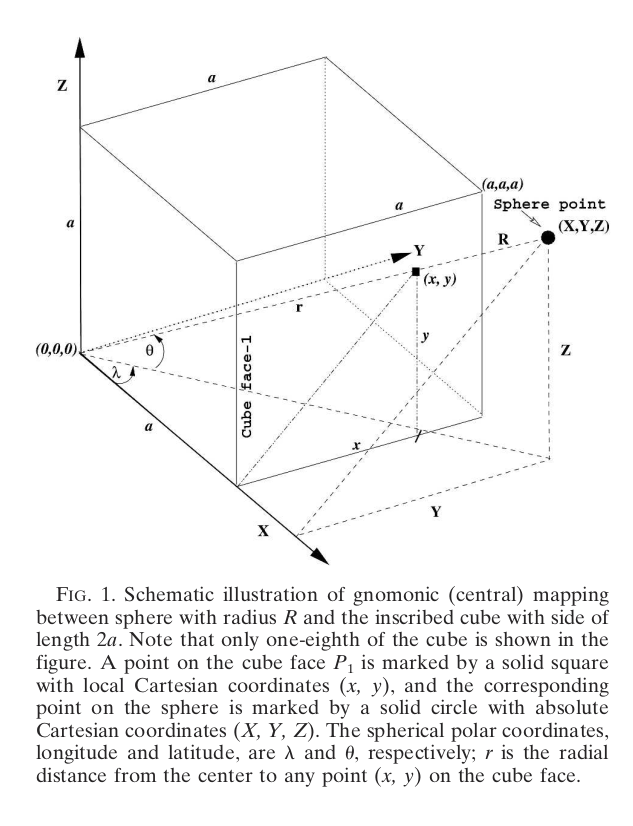
\includegraphics[scale=0.4,trim=0cm 9cm 0cm 0cm, clip]{CLIMA-atmos/figures/numerics/NairFig1.png}
    \caption{One octant of inscribed cube and one quadrant of cube face $P_1$ (from \cite{Nair2005}). Note that $(X,Y,Z)$ in the figure corresponds to $(x,y,z)$ in the text, and $(x,y)$ in the figure corresponds to $(\xi^1,\xi^2)$.}
    \label{fig:NairFig1}
\end{figure}

\begin{figure}
    \centering
    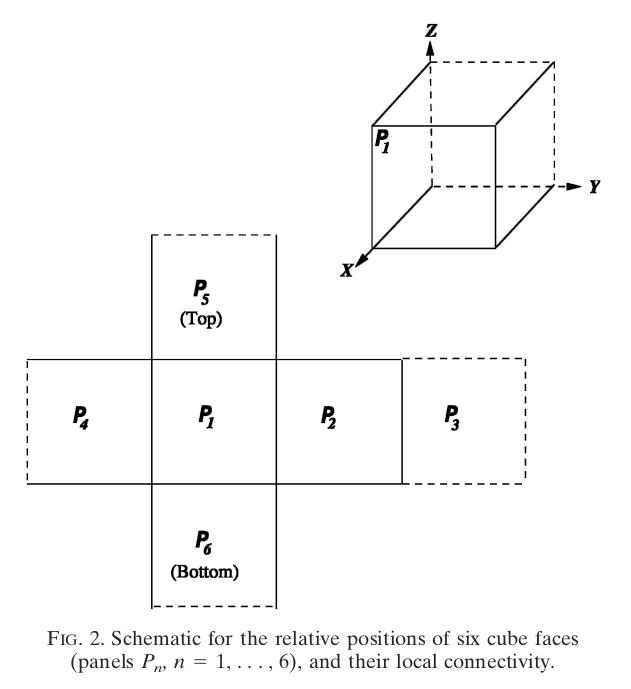
\includegraphics[scale=0.4]{CLIMA-atmos/figures/numerics/NairFig2.png}
    \caption{Relative positions of the six cube faces ($P^n$, $n=1, \dots, 6$) and their local connectivity. (From \cite{Nair2005}. The top-right cube represents only one octant of the cube and one quadrant of the $P^1$ face. The reader should be aware that currently the cube face labelling presented in this figure does not reflect the internal numbering we have in ClimateMachine. }
    \label{fig:NairFig2}
\end{figure}

We assume a Cartesian coordinate system for the Euclidean space in which the sphere and inscribed cube are embedded, with coordinates $(x^1, x^2, x^3) = (x, y, z)$ and associated coordinate vectors directed normal to the faces of the cube; the coordinate origin is at the collocated centers of the cube and sphere (and the $z$ coordinate is not to be confused with the altitude $z$ we defined previously). See Fig.~\ref{fig:NairFig1}. Let $(\xi^1, \xi^2)$ be local coordinates on the surface of each cube face (labeled $n=1,\dots, 6)$,  and let $(\lambda, \phi, r)$ denote the usual spherical polar coordinates with longitude  $\lambda$, latitude $\phi$, and radial distance from the planet center $r=r(\lambda, \phi, \xi^3$). The radius $r$ depends on the horizontal coordinates and a generalized vertical coordinate $\xi^3$. That is, we can view the spherical polar coordinates as functions of the generalized coordinates $(\xi^1, \xi^2, \xi^3, n)$, with longitude $\lambda = \lambda(\xi^1, \xi^2, n)$ and latitude $\phi = \phi(\xi^1, \xi^2, n)$ parameterized by $(\xi^1, \xi^2)$ for each face $n$, and $r = r(\xi^1, \xi^2, \xi^3)$ parameterized by all three generalized coordinates ($r$ will not depend on the face index $n$). Then, we can write the usual transformation from spherical polar coordinates ($\lambda, \phi, r)$ to Cartesian coordinates in the embedding space (as in section~\ref{s:example_coordinates}) as
\begin{subequations} \label{eq:spherical-coords-terrain-follow}
    \begin{align}
    x &= r(\xi^1, \xi^2, \xi^3) \cos \lambda(\xi^1, \xi^2, n) \cos \phi(\xi^1, \xi^2, n) , \\
    y &= r(\xi^1, \xi^2, \xi^3) \sin \lambda(\xi^1, \xi^2, n) \cos \phi(\xi^1, \xi^2, n) , \\
    z &= r(\xi^1, \xi^2, \xi^3) \sin \phi(\xi^1, \xi^2, n).
    \end{align}
\end{subequations}
We adopt the convention that lateral faces of the cube (normal to the $x$ and $y$ axes) are labeled $n=1, \dots, 4$; the top and bottom faces (normal to the $z$ axis) are labeled as $n=5$ and $n=6$, respectively (Fig.~\ref{fig:NairFig2}).

\section{Equidistant Cubed-Sphere Projection}\label{s:cubed_sphere_transform}

\hl{[TS: I non-dimensionalized the cubed sphere coordinates, so that this works without much trouble for a deep atmosphere, with varying $r$. Valeria/Daniel: please check the resulting relations.]}

Let $P^1$ be the cube face with $x$ as the normal direction going from the center through the prime meridian, and consider the first positive octant of the cube. If we adopt local Cartesian coordinates centered on the cube face, so that $(\xi^1, \xi^2) \in [-1, 1]$, the following trigonometric relations hold for $n=1$ (Fig.~\ref{fig:NairFig1}):
\begin{equation}\label{eq:cube-radial-distance-and-coords}
    \sin \phi = \frac{z}{r}, \quad \tan \lambda = \xi^1 = \frac{y}{x}, \quad \text{and} \quad \frac{y}{z} = \frac{\xi^1}{\xi^2}. 
\end{equation}
From the above relations and \eqref{eq:spherical-coords-terrain-follow}, we have that
\begin{subequations} \label{eq:P1-sphere-to-cube}
    \begin{align}
        \xi^1 &= \tan \lambda,\\
        \xi^2 &= \tan \phi \sec \lambda .
    \end{align}
\end{subequations}
Equations \eqref{eq:P1-sphere-to-cube} give the basic gnomonic transformation between the cube and its circumscribing sphere. In this nondimensional form, the transformations from longitude and latitude to the local coordinates $\xi^1$ and $\xi^2$ on the cube faces do not depend on $r$; thus, $(\xi^1, \xi^2)$ parameterize $(\lambda, \phi)$ for any spherical surface of radius $r$.

Relations analogous to \eqref{eq:P1-sphere-to-cube} hold for the other faces of the cube and can be obtained by rotation of the spherical polar coordinate system. Given the mappings $(\xi^1, \xi^2) \rightarrow (\lambda, \phi)$ for the horizontal coordinates on the surface of the spherical shells, we can obtain the mappings for the 3D coordinates $(\xi^2, \xi^2, \xi^3) \rightarrow (x, y, z)$ from \eqref{eq:spherical-coords-terrain-follow}.

To obtain the mappings, we use the nondimensional radial distance $r_c$ from a point with local Cartesian coordinates ($\xi^2, \xi^2$) on the face of the cube to the center of the cube, with  
\[
r_c^2 = 1 + (\xi^1)^2 + (\xi^2)^2.
\]
The results for the 6 cube faces, with $r=r(\xi^1, \xi^2, \xi^3)$ understood to depend on all three generalized coordinates, are as follows \citep[cf.][]{Nair2005}.

\begin{enumerate}
\item For $P^1$ $\left(-\frac{\pi}{4} \leq \lambda \leq  \frac{\pi}{4}, \quad -\frac{\phi}{4} \leq \lambda \leq  \frac{\phi}{4} \right)$: 
\begin{equation}
   \begin{array}{l}
        \xi^1 = \tan \lambda,\\
        \xi^2 = \tan \phi \sec \lambda ,
   \end{array}
\end{equation}
and
\begin{equation}\label{eq:P1-cube-to-global-and-vice-versa}
    \begin{array}{l}
        x = r/r_c,  \\
        y = (r/r_c) \xi^1,\\
        z = (r/r_c) \xi^2,
    \end{array}
    \qquad 
    \begin{array}{l}
         \xi^1 = {y}/{x}, \\
         \xi^2 = {z}/{x} .\\
    \end{array}
\end{equation}
% and
% \begin{equation}
% \vec{b}_1 = 
%     \begin{bmatrix}
%         r\frac{-\xi^1}{r_c^3} + \frac{\partial r}{\partial \xi^1}\frac{1}{r_c}  \\
%         r(\frac{1}{r_c} - \frac{(\xi^1)^2}{r_c^3})+ \frac{\partial r}{\partial \xi^1}\frac{\xi^1}{r_c} \\
%         r( - \frac{\xi^1 \xi^2}{r_c^3})+ \frac{\partial r}{\partial \xi^2}\frac{\xi^2}{r_c} \\
%     \end{bmatrix}
% \qquad 
% \vec{b}_2 = 
%     \begin{bmatrix}
%         r\frac{-\xi^2}{r_c^3} + \frac{\partial r}{\partial \xi^2}\frac{1}{r_c}  \\
%         r( - \frac{\xi^1 \xi^2}{r_c^3})+ \frac{\partial r}{\partial \xi^2}\frac{\xi^1}{r_c} \\
%         r(\frac{1}{r_c} - \frac{(\xi^2)^2}{r_c^3})+ \frac{\partial r}{\partial \xi^2}\frac{\xi^2}{r_c} \\
%     \end{bmatrix}
% \qquad 
% \vec{b}_3 = 
%     \begin{bmatrix}
%         \frac{\partial r}{\partial \xi^3}\frac{1}{r_c}  \\
%         \frac{\partial r}{\partial \xi^3}\frac{\xi^1}{r_c}\\
%         \frac{\partial r}{\partial \xi^3}\frac{\xi^2}{r_c}\\
%     \end{bmatrix}
% \end{equation}

\item For $P^2$ $\left(\frac{\pi}{4} \leq \lambda \leq  \frac{3\pi}{4}, \quad -\frac{\phi}{4} \leq \lambda \leq  \frac{\phi}{4} \right)$:
\begin{equation}
\begin{split} \label{eq:P2-sphere-to-cube}
        \xi^1 &= - \cot \lambda ,\\
        \xi^2 &= \tan \phi \csc \lambda ,
\end{split}
\end{equation}
and
\begin{equation}\label{eq:P2-cube-to-global-and-vice-versa}
    \begin{array}{l}
        x = -(r/r_c) \xi^1 , \\
        y = (r/r_c),\\
        z = (r/r_c) \xi^2,
    \end{array}
\qquad
    \begin{array}{l}
        \xi^1 = -{x}/{y}, \\
        \xi^2 =  {z}/{y} .\\
    \end{array}
\end{equation}
% and
% \begin{equation}
% \vec{b}_1 = 
%     \begin{bmatrix}
%         -r(\frac{1}{r_c} - \frac{(\xi^1)^2}{r_c^3}) -\frac{\partial r}{\partial \xi^1}\frac{\xi^1}{r_c} \\
%         r\frac{-\xi^1}{r_c^3} + \frac{\partial r}{\partial \xi^1}\frac{1}{r_c}  \\
%         r( - \frac{\xi^1 \xi^2}{r_c^3})+ \frac{\partial r}{\partial \xi^2}\frac{\xi^2}{r_c} \\
%     \end{bmatrix}
% \qquad 
% \vec{b}_2 = 
%     \begin{bmatrix}
%         -r( - \frac{\xi^1 \xi^2}{r_c^3}) - \frac{\partial r}{\partial \xi^2}\frac{\xi^1}{r_c} \\
%         r\frac{-\xi^2}{r_c^3} + \frac{\partial r}{\partial \xi^2}\frac{1}{r_c}  \\
%         r(\frac{1}{r_c} - \frac{(\xi^2)^2}{r_c^3})+ \frac{\partial r}{\partial \xi^2}\frac{\xi^2}{r_c} \\
%     \end{bmatrix}
% \qquad 
% \vec{b}_3 = 
%     \begin{bmatrix}
%         -\frac{\partial r}{\partial \xi^3}\frac{\xi^1}{r_c}\\
%         \frac{\partial r}{\partial \xi^3}\frac{1}{r_c}  \\
%         \frac{\partial r}{\partial \xi^3}\frac{\xi^2}{r_c}\\
%     \end{bmatrix}
% \end{equation}
\item For $P^3$ $\left(\frac{3\pi}{4} \leq \lambda \leq  \frac{5\pi}{4}, \quad -\frac{\phi}{4} \leq \lambda \leq  \frac{\phi}{4} \right)$:
\begin{equation} \label{eq:P3-sphere-to-cube}
    \begin{array}{l}
        \xi^1 = - \tan \lambda ,\\
        \xi^2 = - \tan \phi \sec \lambda ,
    \end{array}
\end{equation}
and
\begin{equation}\label{eq:P3-cube-to-global-and-vice-versa}
    \begin{array}{l}
        x = -(r/r_c),  \\
        y = -(r/r_c) \xi^1,\\
        z = (r/r_c) \xi^2,
    \end{array}
    \qquad 
    \begin{array}{l}
        \xi^1 = {y}/{x}, \\
        \xi^2 = - {z}/{x} .\\
    \end{array}
\end{equation}
% and
% \begin{equation}
% \vec{b}_1 = 
%     \begin{bmatrix}
%         -r\frac{-\xi^1}{r_c^3} - \frac{\partial r}{\partial \xi^1}\frac{1}{r_c}  \\
%         -r(\frac{1}{r_c} - \frac{(\xi^1)^2}{r_c^3})- \frac{\partial r}{\partial \xi^1}\frac{\xi^1}{r_c} \\
%         r( - \frac{\xi^1 \xi^2}{r_c^3})+ \frac{\partial r}{\partial \xi^2}\frac{\xi^2}{r_c} \\
%     \end{bmatrix}
% \qquad 
% \vec{b}_2 = 
%     \begin{bmatrix}
%         -r\frac{-\xi^2}{r_c^3} - \frac{\partial r}{\partial \xi^2}\frac{1}{r_c}  \\
%         -r( - \frac{\xi^1 \xi^2}{r_c^3})- \frac{\partial r}{\partial \xi^2}\frac{\xi^1}{r_c} \\
%         r(\frac{1}{r_c} - \frac{(\xi^2)^2}{r_c^3})+ \frac{\partial r}{\partial \xi^2}\frac{\xi^2}{r_c} \\
%     \end{bmatrix}
% \qquad 
% \vec{b}_3 = 
%     \begin{bmatrix}
%         -\frac{\partial r}{\partial \xi^3}\frac{1}{r_c}  \\
%         -\frac{\partial r}{\partial \xi^3}\frac{\xi^1}{r_c}\\
%         \frac{\partial r}{\partial \xi^3}\frac{\xi^2}{r_c}\\
%     \end{bmatrix}
% \end{equation}


\item For $P^4$ $\left(\frac{5\pi}{4} \leq \lambda \leq  \frac{7\pi}{4}, \quad -\frac{\phi}{4} \leq \lambda \leq  \frac{\phi}{4} \right)$:
\begin{equation} \label{eq:P4-sphere-to-cube}
    \begin{array}{l}
        \xi^1 = - \cot \lambda ,\\
        \xi^2 = - \tan \phi \csc \lambda ,
    \end{array}
\end{equation}
and
\begin{equation}\label{eq:P4-cube-to-global-and-vice-versa}
    \begin{array}{l}
        x = (r/r_c) \xi^1,  \\
        y = -(r/r_c),\\
        z = (r/r_c) \xi^2,
    \end{array}
    \qquad
    \begin{array}{l}
        \xi^1 = -{x}/{y}, \\
        \xi^2 = -{z}/{y} .\\
    \end{array}
\end{equation}
% and
% \begin{equation}
% \vec{b}_1 = 
%     \begin{bmatrix}
%         r(\frac{1}{r_c} - \frac{(\xi^1)^2}{r_c^3}) +\frac{\partial r}{\partial \xi^1}\frac{\xi^1}{r_c} \\
%         -r\frac{-\xi^1}{r_c^3} - \frac{\partial r}{\partial \xi^1}\frac{1}{r_c}  \\
%         r( - \frac{\xi^1 \xi^2}{r_c^3})+ \frac{\partial r}{\partial \xi^2}\frac{\xi^2}{r_c} \\
%     \end{bmatrix}
% \qquad 
% \vec{b}_2 = 
%     \begin{bmatrix}
%         r( - \frac{\xi^1 \xi^2}{r_c^3}) + \frac{\partial r}{\partial \xi^2}\frac{\xi^1}{r_c} \\
%         -r\frac{-\xi^2}{r_c^3} + \frac{\partial r}{\partial \xi^2}\frac{1}{r_c}  \\
%         r(\frac{1}{r_c} - \frac{(\xi^2)^2}{r_c^3})+ \frac{\partial r}{\partial \xi^2}\frac{\xi^2}{r_c} \\
%     \end{bmatrix}
% \qquad 
% \vec{b}_3 = 
%     \begin{bmatrix}
%         \frac{\partial r}{\partial \xi^3}\frac{\xi^1}{r_c}\\
%         -\frac{\partial r}{\partial \xi^3}\frac{1}{r_c}  \\
%         \frac{\partial r}{\partial \xi^3}\frac{\xi^2}{r_c}\\
%     \end{bmatrix}
% \end{equation}

\item For $P^5$ $\left(\pi/4 \leq \phi \leq \pi/2 \right)$:
\begin{equation} \label{eq:P5-sphere-to-cube}
    \begin{array}{l}
        \xi^1 = - \sin \lambda \cot \phi ,\\
        \xi^2 = - \cos \lambda \cot \phi , 
    \end{array}
\end{equation}
and
\begin{equation}\label{eq:P5-cube-to-global-and-vice-versa}
    \begin{array}{l}
        x = - (r/r_c) \xi^2,  \\
        y = (r/r_c) \xi^1,\\
        z = (r/r_c),
    \end{array}
    \qquad
    \begin{array}{l}
        \xi^1 = {y}/{z}, \\
        \xi^2 = -{x}/{z} .\\
    \end{array}
\end{equation}
% and
% \begin{equation}
% \vec{b}_1 = 
%     \begin{bmatrix}
%         -r( - \frac{\xi^1 \xi^2}{r_c^3})- \frac{\partial r}{\partial \xi^2}\frac{\xi^2}{r_c} \\
%         r(\frac{1}{r_c} - \frac{(\xi^1)^2}{r_c^3}) +\frac{\partial r}{\partial \xi^1}\frac{\xi^1}{r_c} \\
%         r\frac{-\xi^1}{r_c^3} + \frac{\partial r}{\partial \xi^1}\frac{1}{r_c}  \\
%     \end{bmatrix}
% \qquad 
% \vec{b}_2 = 
%     \begin{bmatrix}
%         -r(\frac{1}{r_c} - \frac{(\xi^2)^2}{r_c^3}) - \frac{\partial r}{\partial \xi^2}\frac{\xi^2}{r_c} \\
%         r( - \frac{\xi^1 \xi^2}{r_c^3}) + \frac{\partial r}{\partial \xi^2}\frac{\xi^1}{r_c} \\
%         r\frac{-\xi^2}{r_c^3} + \frac{\partial r}{\partial \xi^2}\frac{1}{r_c}  \\
%     \end{bmatrix}
% \qquad 
% \vec{b}_3 = 
%     \begin{bmatrix}
%         -\frac{\partial r}{\partial \xi^3}\frac{\xi^2}{r_c}\\
%         \frac{\partial r}{\partial \xi^3}\frac{\xi^1}{r_c}\\
%         \frac{\partial r}{\partial \xi^3}\frac{1}{r_c}  \\
%     \end{bmatrix}
% \end{equation}

\item For $P^6$ $\left(-\pi/2 \leq \phi \leq -\pi/4 \right)$:
\begin{equation} \label{eq:P6-sphere-to-cube}
    \begin{array}{l}
        \xi^1 = - \sin \lambda \cot \phi ,\\
        \xi^2 = -\cos \lambda \cot \phi ,
    \end{array}
\end{equation}
and
\begin{equation}\label{eq:P6-cube-to-global-and-vice-versa}
    \begin{array}{l}
        x = (r/r_c) \xi^2,  \\
        y = (r/r_c)\xi^1,\\
        z = -(r/r_c),
    \end{array}
    \qquad
    \begin{array}{l}
        \xi^1 = -{y}/{z}, \\
        \xi^2 = -{x}/{z}. \\
    \end{array}
\end{equation}
% and
% \begin{equation}
% \vec{b}_1 = 
%     \begin{bmatrix}
%         r( - \frac{\xi^1 \xi^2}{r_c^3})+ \frac{\partial r}{\partial \xi^2}\frac{\xi^2}{r_c} \\
%         r(\frac{1}{r_c} - \frac{(\xi^1)^2}{r_c^3}) +\frac{\partial r}{\partial \xi^1}\frac{\xi^1}{r_c} \\
%         -r\frac{-\xi^1}{r_c^3} - \frac{\partial r}{\partial \xi^1}\frac{1}{r_c}  \\
%     \end{bmatrix}
% \qquad 
% \vec{b}_2 = 
%     \begin{bmatrix}
%         r(\frac{1}{r_c} - \frac{(\xi^2)^2}{r_c^3}) + \frac{\partial r}{\partial \xi^2}\frac{\xi^2}{r_c} \\
%         r( - \frac{\xi^1 \xi^2}{r_c^3}) + \frac{\partial r}{\partial \xi^2}\frac{\xi^1}{r_c} \\
%         -r\frac{-\xi^2}{r_c^3} + \frac{\partial r}{\partial \xi^2}\frac{1}{r_c}  \\
%     \end{bmatrix}
% \qquad 
% \vec{b}_3 = 
%     \begin{bmatrix}
%         \frac{\partial r}{\partial \xi^3}\frac{\xi^2}{r_c}\\
%         \frac{\partial r}{\partial \xi^3}\frac{\xi^1}{r_c}\\
%         -\frac{\partial r}{\partial \xi^3}\frac{1}{r_c}  \\
%     \end{bmatrix}
% \end{equation}
\end{enumerate}

In this nondimensional form, it is clear the $(\xi^1, \xi^2)$ parameterize the horizontal spherical coordinates $(\lambda, \phi)$, whereas $r = r(\xi^1, \xi^2, \xi^3)$ is the radial (vertical) coordinate. 

\section{Equiangular Cubed Sphere}

An alternative parameterization of the horizontal spherical coordinates $(\lambda, \phi)$ follows from the equiangular projection that employs central angles $(\alpha, \beta)$ as coordinates,
\begin{align}
    \begin{array}{l}
        \xi^1 = \tan{\alpha}, \\
        \xi^2 = \tan{\beta} , \\
    \end{array}
\end{align}
with $\alpha, \beta \in [- \pi/4, \pi/4]$. Uniformly discretizing $(\alpha, \beta)$ results in a more uniform distribution of grid points on the sphere than uniformly discretizing the equidistant cubed sphere coordinates $(\xi^1, \xi^2)$; hence, the equiangular projection is preferable \citep{Rancic1996, Nair2005}. Where we use it, we simply use the relations in chapter~\ref{ch:gov_equations} with $(\xi^1, \xi^2) = (\alpha, \beta)$.



\section{Metrics on the Cubed Sphere}
\label{sec:metrics-cubed-sphere}
To compute the metric tensors for the cubed-sphere coordinates $(\xi^1, \xi^2, \xi^3)$, consider an arbitrary position vector $\vec{r}$, defined in terms of the absolute Cartesian coordinates $(x,y,z)$, such that $d\vec{r} = (dx, dy, dz)$. Following Chapter~\ref{ch:gov_equations}, we can define the position vector $\vec{r}$ in terms of the covariant basis vectors 
\begin{equation}
    \vec{b}_1 = \frac{\partial \vec{r}}{\partial \xi^1}, \qquad
    \vec{b}_2 = \frac{\partial \vec{r}}{\partial \xi^2}, \quad \text{and} \quad
    \vec{b}_3 = \frac{\partial \vec{r}}{\partial \xi^3}.
\end{equation}

The covariant metric tensor consists of components $g_{ij} = \vec{b}_i \cdot \vec{b}_j$. From the relations in section~\ref{s:cubed_sphere_transform}, it is 
\begin{align}\label{eq:metric-tensor-from-cube-to-sphere}
    g_{ij}  =
        \frac{r^2}{r_c^4}
     \left[ 
         \begin{array}{ccc}
              1^2 + (\xi^2)^2 & - \xi^1\xi^2 & 0\\
               & 1^2 + (\xi^1)^2 & 0\\
              && 0
         \end{array}
     \right]
    + \left[ 
        \begin{array}{ccc}
             \big(\frac{\partial r}{\partial \xi^1}\big)^2 
             & \big(\frac{\partial r}{\partial \xi^1}\big)\big(\frac{\partial r}{\partial \xi^2}\big) 
             & \big(\frac{\partial r}{\partial \xi^1}\big)\big(\frac{\partial r}{\partial \xi^3}\big) \\
             & \big(\frac{\partial r}{\partial \xi^2}\big)^2 
             & \big(\frac{\partial r}{\partial \xi^2}\big)\big(\frac{\partial r}{\partial \xi^3}\big) \\
             &
             &\big(\frac{\partial r}{\partial \xi^3}\big)^2
        \end{array}
    \right],
\end{align}
with the lower triangles completed by symmetry.
Note that the same metric tensor $g_{ij}$ is used on all the cube faces, irrespective of their local transformations.

When there is no topography, namely $r = r(\xi^3)$, the metric tensor becomes that in~\cite{Nair2005}.
\begin{align}\label{eq:metric-tensor-from-cube-to-sphere-2}
    g_{ij} =
    \frac{r^2}{r_c^4}
    \left[ 
        \begin{array}{cc}
             1^2 + (\xi^2)^2 & - \xi^1\xi^2 \\
             - \xi^1\xi^2    & 1^2 + (\xi^1)^2
        \end{array}
    \right].
\end{align}
The determinant of \eqref{eq:metric-tensor-from-cube-to-sphere-2} is $\det(g_{ij}) = r^2 / r^2_c \Rightarrow |\det(g_{ij})|^{1/2} = r / r_c$.
For the equiangular projection, the metric tensor in this case is

\begin{align}
    g_{ij} =
    \frac{R^2}{\delta^4 \cos^2 \alpha \cos^2 \beta}
    \left[ 
        \begin{array}{cc}
             1 + \tan^2 \alpha        & - \tan \alpha \tan \beta \\
             - \tan \alpha \tan \beta & 1 + \tan^2 \beta 
        \end{array}
    \right],
\end{align}

\noindent where we have used $\delta^2 = 1 + \tan^2 \alpha + \tan^2 \beta$.

\section[Vector and Velocity Transform]{Vector and Velocity Transform}
% \hl{[TS: Daniel, the main thing we'll need is transformations between covariant velocities $u_i$ on the cubed sphere and local Cartesian velocities on the sphere ($u, v, w$), that is, between the cubed-sphere velocities and the physical components $g_{s, ii}^{1/2} u_s^i$ (no summation) on the sphere, where $u_s^i$ are the spherical coordinate velocity components ($u/(r \cos\phi), v/r, w)$ and $g_{s, ii}$ is the spherical-coordinate metric tensor.]}
% \hl{Should we use contravariant velocity? I compute it by first transforming to global Cartesian velocity then spherical velocity and scaling to local  Cartesian velocity [TS: Writing down covariant velocities is easier, and I think it's easiest to start from the local Cartesian velocities $(u, v, w)$ we are all familiar with. That is, take $(u, v, w)$ (eastward, northward, upward) as given and transform to covariant $u_i$.]}

The transformation matrices related to changing velocity in different coordinate systems can be obtained from aforementioned metrics.


The transformation between covariant~($u_i$) and contravariant~($u^i$) velocities in the cubed-sphere coordinates is
\[u_i =  g_{ij} u^j \]
here $g_{ij}$ are in~\eqref{eq:metric-tensor-from-cube-to-sphere}.

The transformation between contravariant~($u^i$) velocities in the cubed-sphere coordinates to the velocities in the global Cartesian coordinate $(x, y, z)$ is
\begin{align*} 
\begin{bmatrix}
             u^{x} \\ u^{y} \\ u^{z}
        \end{bmatrix}  
        = \begin{bmatrix}
             \vec{b}_{1} & \vec{b}_{2} & \vec{b}_{3}
             \end{bmatrix} 
             \begin{bmatrix}
             u^{1} \\ u^{2} \\ u^{3}
        \end{bmatrix}
\end{align*}
where $\vec{b}_i$ are defined in section~\ref{sec:metrics-cubed-sphere}.

The transformation between contravariant~($u^i$) velocities in the cubed-sphere coordinates to the angular velocities in the spherical coordinate $(\lambda, \phi, r)$ is
\begin{align*}
\begin{bmatrix}
             u^{\lambda} \\ u^{\phi} \\ u^{r}
        \end{bmatrix}  
        =
        \begin{bmatrix}
             \vec{b}_{\lambda} & \vec{b}_{\phi} & \vec{b}_{r}
        \end{bmatrix}^{-1}
        \begin{bmatrix}
             \vec{b}_{1}&  \vec{b}_{2}& \vec{b}_{3}
        \end{bmatrix}
        \begin{bmatrix}
             u^{1} \\ u^{2} \\ u^{3}
        \end{bmatrix}
\end{align*}
where (See~\eqref{e:spherical_polar_coordinates})
\begin{align*}
\begin{bmatrix}
\vec{b}_{\lambda} & \vec{b}_{\phi} & \vec{b}_{r}
\end{bmatrix}^{-1} 
= 
\begin{bmatrix}
-\frac{\sin \lambda}{r\cos\phi} & \frac{\cos \lambda}{r\cos\phi} & 0 \\
-\frac{\sin \phi\cos\lambda}{r} & -\frac{\sin\phi\sin  \lambda}{r} & \frac{\cos \phi}{r} \\
\cos\phi\cos\lambda & \cos\phi\sin\lambda  & \sin\phi \\
\end{bmatrix}
\end{align*}

The transformation between contravariant velocities $u^i$ on the cubed sphere and local Cartesian velocities ($u, v, w$), namely eastward, northward, upward velocities, is
\begin{align*}
\begin{bmatrix}
             u \\ v \\ w
        \end{bmatrix} 
        &= \begin{bmatrix}
             r\cos\phi &  &\\
              & r & \\
              &  & 1
        \end{bmatrix}
        \begin{bmatrix}
             \vec{b}_{\lambda} & \vec{b}_{\phi} & \vec{b}_{r}
        \end{bmatrix}^{-1}
        \begin{bmatrix}
             \vec{b}_{1}&  \vec{b}_{2}& \vec{b}_{3}
        \end{bmatrix}
        \begin{bmatrix}
             u^{1} \\ u^{2} \\ u^{3}
        \end{bmatrix} \\
        &= 
        \begin{bmatrix}
-\sin \lambda & \cos \lambda & 0 \\
-\sin \phi\cos\lambda & -\sin\phi\sin  \lambda & \cos \phi \\
\cos\phi\cos\lambda & \cos\phi\sin\lambda  & \sin\phi \\
\end{bmatrix}
        \begin{bmatrix}
             \vec{b}_{1}&  \vec{b}_{2}& \vec{b}_{3}
        \end{bmatrix}
        \begin{bmatrix}
             u^{1} \\ u^{2} \\ u^{3}
        \end{bmatrix}
\end{align*}

These velocity transformations are equally applicable for any vector field transformations between different coordinate systems.

% The matrix 
% The spherical velocity $(u,v)$ is written in terms of $(u^1, u^2)$ using \eqref{eq:v-in-terms-of-u}, as follows
% \begin{align}\label{eq:dual-transformations}
%     \left[ 
%         \begin{array}{c}
%              u \\
%              v
%         \end{array}
%     \right] = 
%         \boldsymbol{B}
%     \left[ 
%         \begin{array}{c}
%              u^{1} \\
%              u^{2}
%         \end{array}
%     \right] , \qquad
%         \left[ 
%         \begin{array}{c}
%              u^{1} \\
%              u^{2}
%         \end{array}
%     \right] =
%     \boldsymbol{B}^{-1}
%     \left[ 
%         \begin{array}{c}
%              u \\
%              v
%         \end{array}
%     \right],
% \end{align}

% \noindent where $\boldsymbol{B}$ is such that $g_{ij} = \boldsymbol{B}^T \boldsymbol{B}$, and $\boldsymbol{B}$ and $\boldsymbol{B}^{-1}$ are interpreted as the ``cube-to-sphere'' and ``sphere-to-cube'' transformation matrices, respectively. The entries of the matrix $\boldsymbol{B}$ depend on the central projection method chosen (e.g., an equiangular or an equidistant projection), local transformation laws and local coordinates. 


\section[Treatment of Vectors Along the Cube-Face Edges]{Treatment of Vectors Along the Cube-Face Edges}
\hl{Is the idea here rotating to some global coordinate system first? 
For the global coordinate, do we use the global Cartesian or global spherical ? Valeria: You can see it this way, or the way I see it from how Nair et al. and also} \citep{Taylor1997} \hl{exposed it is that since degrees of freedom along cube face edges wouldn't have a unique representation in terms of a unique coordinate system, because they share two panels (faces) of the cube, you express only those in an intermediate representation that is common to both panels and is free of singularities. For this reason, the lat-long one is a suitable representation. Hence, when you want to express a vector quantity and you want this to have a well-posed representation, you can transform its coordinates from panel A, to spherical and from spherical to panel B. In practice, when implementing this, only one step is required if all degrees of freedom along the cube edges are already expressed in terms of lat-long. Hence, you would transform only (lat,long) $\rightarrow $ panel P, whatever panel P's state vector degrees of freedom you are advancing your solution of.}
The treatment of vector quantities such as flux terms requires special attention along cube edges, because the contiguous faces of the cube employ different local coordinate systems. Consider two adjoining elements separated by a cube edge and belonging to the cube faces $P^n$ and $P^l$, such that $n, l \in {1, \ldots , 6}$ and $n \neq l$. Let $(F^{-}_n, G^{-}_n)$ and $(F^{+}_n, G^{+}_n)$ be the left and right vectors located at a common point (an LGL point) but having two different local coordinate systems. In the case of flux vectors, $\boldsymbol{\mathcal{F}}$, we could use the notation $\boldsymbol{\mathcal{F}}^{\pm} = \boldsymbol{\mathcal{F}}(U^{\pm})$ and $\boldsymbol{\mathcal{G}}^{\pm} = \boldsymbol{\mathcal{G}}(U^{\pm})$. To compute numerical fluxes in the $\xi^1$ direction across the edge of $P^n$ in a DG discretization, but even to ensure continuity across cube edges in a CG formulation, both the \emph{left} and \emph{right} components, $F^{-}_n$ and $F^{+}_n$, respectively, are required. The right component $F^{+}_n$ is computed from $(F^{+}_l, G^{+}_l)$ by the procedure described below.

First, transform $(F^{+}_l, G^{+}_l)$ defined on $P^l$ into the corresponding spherical components $(F^{+}_s, G^{+}_s)$ by applying the matrix $\vec{B}_l$. Next, transform $(F^{+}_s, G^{+}_s)$ into $(F^{+}_n, G^{+}_n)$ defined on $P^n$ by applying the inverse matrix $\vec{B}^{-1}$. The dual transformations based on \eqref{eq:dual-transformations} are summarized below:

\begin{align}
\textrm{Step 1.} \qquad
    \left[ 
        \begin{array}{c}
             F^{+}_s \\
             G^{+}_s
        \end{array}
    \right] = 
        \boldsymbol{B}_l
    \left[ 
        \begin{array}{c}
             F^{+}_l \\
             G^{+}_l
        \end{array}
    \right],
\end{align}

\begin{align}
\textrm{Step 2.} \qquad
    \left[ 
        \begin{array}{c}
             F^{+}_n \\
             G^{+}_n
        \end{array}
    \right] = 
        \boldsymbol{B}^{-1}_n
    \left[ 
        \begin{array}{c}
             F^{+}_s \\
             G^{+}_s
        \end{array}
    \right],
\end{align}

\begin{align}
\textrm{Combined:} \qquad 
\Rightarrow
    \left[ 
        \begin{array}{c}
             F^{+}_n \\
             G^{+}_n
        \end{array}
    \right] = 
        \boldsymbol{B}^{-1}_n\boldsymbol{B}_l
    \left[ 
        \begin{array}{c}
             F^{+}_l \\
             G^{+}_l
        \end{array}
    \right]
\end{align}

\noindent This procedure extends to any pair of cube faces and transformation matrices, and dual transformation matrices $\boldsymbol{B}^{-1}_n\boldsymbol{B}_l$ can be precomputed.

When using an equiangular transformation, the angles $(\alpha,\beta)$ are the independent variables instead of the local $(\xi^1, \xi^2)$ on the cube faces. For an equiangular projection, the basis vectors introduced right after \eqref{eq:metric-tensor-from-cube-to-sphere}, $\vec{r}_1 = \vec{r}_\alpha$ and $\vec{r}_2 =\vec{r}_{\beta} $ may be written as

\begin{subequations}
    \begin{align}
        \vec{r}_{\alpha} &= \frac{l}{cos^2 \alpha} \vec{r}_{\xi^1} ,\\
        \vec{r}_{\beta} &= \frac{l}{cos^2 \beta} \vec{r}_{\xi^2},
    \end{align}
\end{subequations}

\noindent where $ \vec{r}_{\xi^1}$ and $ \vec{r}_{\xi^2}$ are defined as follows. We emphasize here the use spherical coordinates $(\lambda, \phi)$ rather than the absolute Cartesian coordinates $(x,y,z)$. For any horizontal vector $\vec r$ on the sphere, we have the following differential form

\begin{align}
    d \vec{r} = \vec{i} r \cos \phi \, d \lambda + \vec{j} r \, d \phi,
\end{align}

\noindent where the vector is decomposed into the east $(\lambda)$ and the north $(\phi)$ directions. The basis vectors can then be expressed as

\begin{subequations}\label{eq:basis-vecs-spherical-wrt-cube}
    \begin{align}
        \vec{b}_{1} &= \vec{r}_{\xi^1} = \vec{i} r \cos \phi \frac{d\lambda}{d \xi^1} + \vec{j} r \frac{d \phi}{d \xi^1},\\
        \vec{b}_{2} &= \vec{r}_{\xi^2} = \vec{i} r \cos \phi \frac{d\lambda}{d \xi^2} + \vec{j} r \frac{d \phi}{d \xi^2} .
    \end{align}
\end{subequations}

When the central angels $\alpha, \beta \in [- \pi / 4, \pi / 4]$ are independent variables instead of local Cartesian coordinates $(\xi^1, \xi^2)$ on the cube faces, we can write the basis vectors using the central equiangular projection:

\begin{align}
    \vec{r}_{\alpha} &= \frac{1}{\cos^2 \alpha} \vec{r}_{\xi^1} \\
    \vec{r}_{\beta}  &= \frac{1}{\cos^2  \beta} \vec{r}_{\xi^2}
\end{align}

\noindent where we use $\vec{r}_{\xi^1}$ and $\vec{r}_{\xi^2}$ as defined in \eqref{eq:basis-vecs-spherical-wrt-cube}.

Furthermore, in this case, the metric tensor can be derived as 

\begin{align}
    g_{ij} =
    \left[ 
        \begin{array}{cc}
             \vec{r}_{\alpha} \cdot \vec{r}_{\alpha} & \vec{r}_{\alpha} \cdot \vec{r}_{\beta} \\
             \vec{r}_{\beta} \cdot \vec{r}_{\alpha} & \vec{r}_{\beta} \cdot \vec{r}_{\beta}
        \end{array}
    \right] =
    \frac{r^2}{\delta^4 \cos^2 \alpha \cos^2 \beta}
    \left[ 
        \begin{array}{cc}
             1 + \tan^2 \alpha        & - \tan \alpha \tan \beta \\
             - \tan \alpha \tan \beta & 1 + \tan^2 \beta 
        \end{array}
    \right] = \widetilde{\vec{B}}^T \widetilde{\vec{B}},
\end{align}

\noindent where the Jacobian of the transformation and the matrix $\widetilde{\vec{B}}$ are, respectively,

\begin{align}
    (\det(\vec{g}_{ij}))^{(1/2)} =
    \frac{r^2}{\delta^3 \cos^2 \alpha \cos^2 \beta},  \quad \textrm{ and } \qquad
    \widetilde{\vec B}=
    \left[ 
        \begin{array}{cc}
             r \cos \phi \lambda_{\alpha}   & r \cos \phi \lambda_{\beta} \\
             r \phi_{\alpha}                & r \phi_{\beta}  
        \end{array}
    \right] .
\end{align}

\noindent The matrices $\widetilde{\vec{B}}$ and $\widetilde{\vec B}^{-1}$ are needed for the transformations between the cube faces and the sphere. So we write them explicitly here

\begin{align}
    \widetilde{\vec{B}} = \vec{B}
    \left[ 
        \begin{array}{cc}
             l / \cos^2{\alpha}   & 0 \\
             0                    & l/ \cos^2{\beta}  
        \end{array}
    \right] , \; \textrm{ and } \qquad
    \widetilde{\vec B}^{-1} =
    \frac{1}{l}
    \left[ 
        \begin{array}{cc}
             \cos^2{\alpha}  & 0 \\
             0               & \cos^2{\beta}  
        \end{array}
    \right] .
\end{align}




%%%%%%%%%%%%%%%%%%%%%%%%%%%%%%%% Space Discretization Chapter %%%%%%%%%%%%%%%%%%%%%%%%%%%%%%%%%%%%%%%%

\chapter{Space Discretization}

\section{Boundary Conditions}

\section{Filters}

All filters (spectral, SGS) need to act on conservable specific quantities, e.g., specific total enthalpy ($h_\mathrm{tot}$, \textbf{not} $\rho e$ etc.). To filter not conservable variables such as pressure and density, only filter fluctuations around hydrostatic reference state (locally computed, ideally).

On curved elements, filters need to conserve mass. This means that in addition to damping the highest modes, we also want the lowest mode to be the same before and after filtering.

\subsection{Hyperviscosity and Hyperdiffusion}

follow \citet{Dennis12a} for CG implementation

\subsection{Spectral Filters}

%%%%%%%%%%%%%%%%%%%%%%%%%%%%%%%%% Time Discretization Chapter %%%%%%%%%%%%%%%%%%%%%%%%%%%%%%%%%%%%%%%%
\chapter{Time Discretization}\label{s:timestepping}

For the atmosphere, the general, compressible equations of motion we use permit a variety of wave modes with different characteristic speeds. Additionally, the equations contain sources that can add stiffness, for example, microphysical processes that occur on timescales of seconds or less. Similarly, stiffness in the land model arises near where the soil reaches saturation and timescales become very short.

The atmosphere equations permit the following wave modes:
\begin{itemize}
    \item Acoustic waves. They have phase speeds around $300~\mathrm{m~s^{-1}}$ in the atmosphere. Density variations and the terms involving pressure in the momentum and energy equations are essential for their existence.
    \item Gravity waves. They have a spectrum of phase speeds. In a deep atmosphere (e.g., in a GCM), the gravest, external mode has phase speed $(gH)^{1/2} \approx 280~\mathrm{m~s^{-1}}$, where $H\approx 8~\mathrm{km}$ is the atmospheric scale height. The gravity term $-\rho \nabla \Phi$ in the momentum equation and the gravitational potential energy $\Phi$ in the energy equation are responsible for their existence.
    \item Inertia-gravity, Rossby waves, and several other wave modes that owe their existence to the Coriolis acceleration $-2\vec{\Omega} \times \rho \vec{u}$ in the momentum equation. They have smaller phase speeds than the acoustic and external gravity waves.
\end{itemize}
Additional stiffness in the equations arises from:
\begin{itemize}
    \item Falling precipitation, whose fall velocity $w_{p,i}$ can reach $10~\mathrm{m~s^{-1}}$ and thus exceeds typical vertical velocities resolved in GCMs.
    \item Microphysical source terms, for example, in the equations for suspended specific humidities $q_k$; they depend on the precipitation specific humidity $q_{p,i}$, which can change rapidly because precipitate falls rapidly. 
    \item SGS diffusive fluxes, whose effective vertical velocity can exceed that of the resolved velocities.
    \item Other parameterized SGS fluxes, for example, convective updrafts, whose vertical velocities can likewise be large.
\end{itemize}
By contrast, radiation evolves on longer timescales than the dynamical quantities and hence, because it is expensive to evaluate, usually is evolved forward in time with longer timesteps than the dynamical quantities. 

We need a stable and computationally efficient time discretization strategy that allows some state vector components to be treated implicitly (e.g., falling precipitation and convective updrafts) and allows other terms (e.g., radiative energy fluxes) to be evaluated less frequently than dynamical terms. In particular, we need a computationally efficient way of handling the physically insignificant acoustic waves.
     
\section{Decomposition of Time Tendencies}

To circumvent the time-step restriction due to the fast acoustic and gravity waves, using implicit-explicit (IMEX) methods is one option. For the LES model, if the aspect ratio of the horizontal ($\Delta_h$) to vertical ($\Delta_v$) grid spacing is near unity, using fully 3D-IMEX methods may be an option.  For LES models with aspect ratios of grid elements $\Delta_h/\Delta_v > 1$ and for global atmospheric models, which generally have $\Delta_h/\Delta_v \gg 1$, we use 1D-IMEX methods in which the time-integrator is fully explicit in the horizontal direction (HE) and implicit in the vertical direction (so-called HEVI schemes). 

IMEX methods require the solution of one or more linear systems at each time step. The linear system is global in 3D, and this may limit scalability of IMEX methods in a multi-node computational setting. In that case, explicit methods in the horizontal, potentially with subcycling of fast terms in a multirate setting, may be a more scalable option to deal with the timestep restrictions. For HEVI schemes, the linear solves are restricted to independent atmospheric columns, which are generally represented on a single compute node. So their scalability across nodes is less restricted.

All of these approaches are based on a decomposition of time tendencies $\Tvector$ into four terms: 
\begin{itemize}
    \item terms to be treated implicitly, labeled by $I$ (the fastest terms);
    \item terms evaluated at the dynamical (advective) timestep, labeled by $d$;
    \item terms to be subcycled $f$ times for each dynamical timestep, labeled by $+f$ (for fast);
    \item terms to be evaluated every $s$ dynamical timesteps, labeled by $-s$ (for slow).
\end{itemize}
With this, we can write the system of ODEs obtained by the space discretization symbolically as
\[
\frac{\partial \vec{Y}}{\partial t} = \Tvector  = \Tvector_{I} + \Tvector_{d} + \Tvector_{+f} + \Tvector_{-s},
\]
where $\vec{Y}$ is a vector of state variables of the model. 

To obtain a linear problem for linear implicit solves, let us linearize the implicit tendency terms $\Tvector_{I}$ by Taylor expansion around a reference state $\vec{Y}_r$,
\begin{equation}\label{e:imex_linearization}
\Tvector_{I}(\vec{Y}) =  \Tvector_I(\vec{Y}_r) + \vec{\mathcal{L}}_I (\vec{Y} - \vec{Y}_r) + \Tvector^N_{I}(\vec{Y}),
\end{equation}
where 
\begin{equation}
    \vec{\mathcal{L}}_I = \left. \frac{\partial\Tvector_I}{\partial\vec{Y}}\right|_{\vec{Y}_r}
\end{equation} 
is the linear component of the tendency operator and $\Tvector^N_{I}(\vec{Y})$ is the nonlinear residual. This then allows us to write the equation of motion \eqref{e:eom_compact} as
\begin{equation}
\label{eq:IMEX}
\frac{\partial\vec{Y}}{\partial t} =  \vec{\mathcal{L}}_I \vec{Y} + \Bigl(\Tvector_I(\vec{Y}_r) - \vec{\mathcal{L}}_I \vec{Y}_r\Bigr) + \Tvector^N_{I}(\vec{Y}) + \Tvector_{d} + \Tvector_{+f} + \Tvector_{-s}.
\end{equation}
Usually, the reference state $\vec{Y}_r$ is chosen so that the tendency of the reference state, $\Tvector_I(\vec{Y}_r)$, and the linear tendency of the reference state, $\vec{\mathcal{L}}_I \vec{Y}_r$, either vanish individually or cancel each other, so that $\Tvector_I(\vec{Y}_r) - \vec{\mathcal{L}}_I \vec{Y}_r=0$. We will justify this in section~\ref{s:IMEX_general}.

\section{Reference State for Linearization}

Solving for the fastest waves implicitly by a linear solve requires linearization of the fastest tendency terms. We generally use reference states characterized by a temperature $T_r(z)$ that may depend on height $z$ but does not depend on horizontal coordinates or time. We enforce hydrostatic balance, and assume the reference state is dry.
%so that the reference state variables are obtained as described in section~\ref{s:initial_conditions} with zero relative humidity ($\mathrm{RH}=0$): the pressure is obtained from \eqref{eq:hydro_pressure}, the density from \eqref{eq:hydro_density}, and the total specific humidity is set to zero, $q_{t,r}=0$.

Because the reference temperature and thus the reference pressure are assumed to be constant in the horizontal, the reference state is assumed at rest, $\vec{u}_r = 0$, consistent with geostrophic balance. Because the reference state is assumed dry, $q_k= 0$ for $k \in \{ t, v, l, i, p\}$ in the reference state.

More sophisticated reference states for linearization are possible, for example, with a latitudinally varying hydrostatically balanced temperature profile, and with a reference velocity in geostrophic and hydrostatic balance with this temperature field. However, we focus on hydrostatic states at rest for now. 
 
 \section{Solving for Acoustic and Gravity Waves Implicitly}
 \label{s:IMEX_general}

Let us lay out in general terms the linearizations for acoustic and gravity waves that underlie IMEX methods in 1D and 3D. The tendency terms responsible for acoustic waves and gravity waves are
 \begin{equation}
 \Tvector_{I}= -\nabla_{1/3} \cdot
 \begin{pmatrix}
 \rho \vec{u} \\
 p \vec{I}_3 \\
 \bigl(e^{\mathrm{tot}} + (\delta_{\mathrm{gw}}-1) \Phi + p/\rho \bigr) \rho \vec{u} \\
 0\\
 \vdots
 \end{pmatrix}
 - \begin{pmatrix}
 0 \\
 \delta_{\mathrm{gw}} \rho \nabla_{1/3} \Phi \\
 0\\
 0\\
 \vdots
 \end{pmatrix},
 \label{eq:3D-imex/tendencies}
 \end{equation}
where all components indicated by dots are zero. The operator $\nabla_{1/3}$ is the 3D differential operator $\nabla_3 = \nabla$ for 3D-IMEX, and it is the 1D operator $\nabla_1 = \vec{k} \partial/\partial_z$ for 1D-IMEX. (The geopotential gradient $\nabla_{1/3} \Phi$ only has a vertical component as long as we consider a spherical planet, so this gradient even in 3D usually only has a vertical component.) The switch $\delta_{\mathrm{gw}}$ (which can only take the value of either $0$ or $1$) is included to indicate whether gravity waves are included in the implicit tendencies: 
\begin{itemize}
    \item $\delta_{\mathrm{gw}}=1$: both acoustic and gravity waves are included in $\Tvector_I$;
    \item $\delta_{\mathrm{gw}}=0$: only acoustic waves are included in $\Tvector_I$.
\end{itemize}

In the tendency \eqref{eq:3D-imex/tendencies}, the terms that need to be linearized are the pressure $p$, which depends nonlinearly on state variables, and the total enthalpy flux $(\rho e^{\mathrm{tot}} + p/\rho) (\rho \vec{u})$. Linearization around a state of rest ($\vec{u}_r=0$) with reference total energy $e^{\mathrm{tot}}_r$, pressure $p_r$, and density $\rho_r$ leads to
 \begin{equation}\label{e:IMEX_linear}
 \vec{\mathcal{L}}_I \vec{Y} = 
 -\nabla_{1/3} \cdot \begin{pmatrix}
 \textcolor{blue}{\rho \vec{u}} \\
 \textcolor{blue}{p_L} \vec{I}_3  \\
 \Bigl(e^{\mathrm{tot}}_r  + (\delta_{\mathrm{gw}}-1)\Phi + p_r/\rho_r \Bigr) \textcolor{blue}{\rho \vec{u}}\\
 0\\
\vdots
\end{pmatrix}
-
\begin{pmatrix}
0 \\
\delta_{\mathrm{gw}} \textcolor{blue} \rho \nabla_{1/3} \Phi \\
0\\
0\\
\vdots
\end{pmatrix}.
\end{equation}
This is linear with respect to \textcolor{blue}{$\rho$} and \textcolor{blue}{$\rho \vec{u}$} (all state variables and linear functions thereof are colored \textcolor{blue}{blue}; all other terms are constants or fixed functions of height $z$). For it to be a linear function of all state variables, the pressure \textcolor{blue}{$p_L$} needs to be expressed as a linear function of state variables. To derive a linear approximation for the pressure, we use the ideal gas law $p = R_m (\rho T)$ and the expression derived from the temperature equation 
%Eq.~\eqref{eq:temperature} 
for $\rho T$ in terms of the internal energy and specific humidities,
\begin{equation}\label{e:pressure}
\begin{split}
p &= R_m (\rho T) \\
  &= \rho R_m T_0 + \frac{R_m}{c_{vm}} \left[\rho e^{\mathrm{tot}} - \rho \Phi - 0.5 \rho \|\vec{u}\|^2 - (\rho q_t - \rho q_l) I_{v,0} + \rho q_i (I_{i,0} + I_{v,0}) \right],
\end{split}
\end{equation}
where we have used the relation $I = e^{\mathrm{tot}} - \Phi - 0.5 \|\vec{u}\|^2$ between total and internal energy. Linearization $p_L = p_r + (\partial p/\partial\vec{Y})\cdot(\vec{Y}-\vec{Y}_r)$ around the reference state $\vec{Y}_r$ with pressure $p_r$ and zero specific humidities leads to 
\begin{equation}\label{eq:pressure_linear}
\textcolor{blue}{p_L} = \textcolor{blue}{\rho} R_d T_0 + \frac{R_d}{c_{vd}} \bigl[ \textcolor{blue}{\rho e^{\mathrm{tot}}} - \textcolor{blue}{\rho} \Phi - (\textcolor{blue}{\rho q_t} - \textcolor{blue}{\rho q_l})I_{v,0} + (\textcolor{blue}{\rho q_i}) (I_{i,0} + I_{v,0}) \bigr].
\end{equation}
If only the total specific humidity $q_t$ is available as a prognostic variable and condensate is determined by saturation adjustment, the condensate specific humidities $q_l$ and $q_i$ in this linearized expression for the pressure can be set to zero. Note that the temperature $T_0$ that appears here is the \emph{reference temperature in the definition of internal energy}, a model constant; it is \emph{not} the temperature $T_r$ of the reference state about which we linearized. In fact, the linearized pressure \eqref{eq:pressure_linear} does not depend on the reference state: the zeroth-order term $p_r$ in the linearization cancels the terms involving the reference state in the linear term, which ensures that the linearized pressure vanishes when the density vanishes. 

We can now see that the sum of the terms involving the reference state in the decomposition \eqref{e:imex_linearization} vanishes,
\[
\Tvector_I(\vec{Y}_r) - \vec{\mathcal{L}}_I \vec{Y}_r = 0.
\]
To see this, it is useful to distinguish the cases when gravity waves are included in the implicit term and when they are not included: 
\begin{itemize}
    \item Acoustic and gravity waves included ($\delta_{\mathrm{gw}}=1$). In this case, it is evident that $\Tvector_I(\vec{Y}_r)=0$ because the pressure gradient ($-\nabla_{1/3} p_r(z)$) and geopotential gradient ($-\rho_r\nabla_{1/3}\Phi$) in the momentum equation (second component of tendency vector) cancel for a hydrostatic reference state with $p_r = p_r(z)$. The same is true for the linear term for a reference state at rest, for which $p_L = p_r$ and $\vec{\mathcal{L}}_I \vec{Y}_r = 0$. 
    \item Only acoustic waves included ($\delta_{\mathrm{gw}}=0$). In this case, neither $\Tvector_I(\vec{Y}_r)$ nor $\vec{\mathcal{L}}_I\vec{Y}_r$ vanish individually, because the geopotential term needed for the cancellation of terms in hydrostatic balance does not appear in the momentum tendency. However, $p_L = p_r$ in a reference state at rest, so that $\Tvector_I(\vec{Y}_r) = \vec{\mathcal{L}}_I\vec{Y}_r$.
\end{itemize}
Thus, in either case, the terms involving the reference state do not appear  in the decomposition \eqref{e:imex_linearization}. 

The nonlinear term follows as the residual 
\begin{equation}\label{e:nonlinear_residual}
\begin{split}
\Tvector^N_{I}(\vec{Y}) & =  \Tvector_I(\vec{Y}) - \vec{\mathcal{L}}_I \vec{Y} \\
& = 
-\nabla_{1/3} \begin{pmatrix}
0 \\
(p - p_L) \vec{I}_3\\
(e^{\mathrm{tot}}  + p/\rho - e^{\mathrm{tot}}_r - p_r/\rho_r) \rho \vec{u}\\
0\\
\vdots
\end{pmatrix}.
\end{split}
\end{equation}
We can verify that the nonlinear residual is small relative to the linear tendency term, as is required for an IMEX approach, as follows. The full pressure (Eq.~\ref{e:pressure}) differs from its linearized counterpart (Eq.~\ref{eq:pressure_linear}) in the inclusion of the kinetic energy term $0.5 \|\vec{u} \|^2$ and of the effects of moisture on the gas constant and specific heat. Relative to the internal energy, the kinetic energy is of order $\|\vec{u}\|^2/c_s^2$ (where $c_s$ is the speed of sound; 
%see section~\ref{s:energy_balance})
and the moisture effects on the gas constant and specific heat are of order $q_t$. Thus, the nonlinear residual $p-p_L$ is small relative to the full pressure $p$: typically of order $10^{-3}$ in Earth's atmosphere. The nonlinear residual in the energy equation depends on the choice of reference state. With a reference temperature $T_r(z)$ that depends on height $z$ only, one may expect $T - T(z) \lesssim 30~\mathrm{K}$ in Earth's atmosphere. Because the internal energy deviation from the reference state dominates the residual $e^{\mathrm{tot}} - e^{\mathrm{tot}}_r$, one may expect a size of the residual $e^{\mathrm{tot}} - e^{\mathrm{tot}}_r$ relative to the full total energy $e^{\mathrm{tot}}$ of order $30~\mathrm{K}/300~\mathrm{K} = 10^{-1}$. Hence, the nonlinear residual in the energy equation is likewise small compared with the linear tendency term. 
 
The decomposition of $\Tvector_I$ up to this point is general and holds for 3D-IMEX and 1D-IMEX, with the appropriate differential operator substituted for $\nabla_{1/3}$.




%-------Bibliography
\bibliographystyle{agufull08}
\bibliography{CLIMA-refs}

\end{document}